%implementing document formatting:
%page setup (page size, text size, page layout, chapters start on a new page).
%memoir is a form of book class that supports any kind of document.
\documentclass[fleqn,a4paper,12pt,twoside,openany,danish]{memoir}

%setting the header and footer in that order:
\setheadfoot{28pt}{28pt} %if any problems are encountered, try changing the latter 28pt with 1cm.

%setting language:
\RequirePackage[danish]{babel}

\usepackage{tocbibind}

%this package makes it possible to treat any element as a float,
%figures and tables are by default treated as floats.
%read http://en.wikibooks.org/wiki/LaTeX/Floats,_Figures_and_Captions to specify your float.
\usepackage{float}
\usepackage{wrapfig}
\usepackage{placeins}
\usepackage{tabu}

%this package makes it possible to make theorems and examples:
\usepackage{amsthm}
%setting the style of examples (parameters: plain, definition, remark):
%(definition is usually used for examples)
\theoremstyle{definition}
%the frist parameter is the syntax used in the document, the second is that which is printed in LaTex.
\newtheorem{example}{Eksempel}

%making it possible to use æ, ø and å:
\usepackage[utf8]{inputenc}
%helps with word division when using æ, ø and å, and makes it ps-font rather than bmp:
\usepackage[T1]{fontenc}

%package for implementation of graphic files:
\usepackage{graphicx}

\usepackage{multirow}

%package for subfigures
%\usepackage{graphicx}
%\usepackage{caption}


%package for captions
\usepackage[nooneline,labelfont=bf]{caption}
%\usepackage{subcaption}

%%package for implementation of math:
\usepackage{amsmath , amsfonts , amssymb, float}

%allowing use of color:
\usepackage{color}
%allowing use of more colors also in tables (see: http://en.wikibooks.org/wiki/LaTeX/Colors):
\usepackage[usenames,dvipsnames,svgnames,table]{xcolor}

%hyperlinks in the tabel of contents - comment this out before the report is printed.
\usepackage{hyperref}
\hypersetup{
%	bookmarks = true,  % Show 'bookmark'-frame in pdf.
	colorlinks = true, % True = colored links, False = framed links.
	citecolor = black,  % Link color for references.
	linkcolor = black,  % Link color in table of contents.
	urlcolor = black,   % Link color for extern URLs.
}

%makes it possible to refer to the name of a chapter rather than just the number.
\usepackage{nameref}

%package for the SI unit standard
\usepackage{siunitx}
\usepackage{units}

%package for writing program code in latex
\usepackage{listings}

\lstset{ 
language=C,               	 	% choose the language of the code
basicstyle=\footnotesize,       % the size of the fonts that are used for the code
numbers=left,                   % where to put the line-numbers
numberstyle=\footnotesize,      % the size of the fonts that are used for the line-numbers
stepnumber=1,                   % the step between two line-numbers. If it is 1 each line will be numbered
numbersep=5pt,                  % how far the line-numbers are from the code
backgroundcolor=\color{white},  % choose the background color. You must add \usepackage{color}
showspaces=false,               % show spaces adding particular underscores
showstringspaces=false,         % underline spaces within strings
showtabs=false,                 % show tabs within strings adding particular underscores
frame=single,           		% adds a frame around the code
tabsize=2,          			% sets default tabsize to 2 spaces
captionpos=b,           		% sets the caption-position to bottom
breaklines=true,       			% sets automatic line breaking
breakatwhitespace=false,    	% sets if automatic breaks should only happen at whitespace
escapeinside={\%*}{*)}          % if you want to add a comment within your code
}

%setting references (using numbers) and supporting i.a. Chicargo-style:
\usepackage{etex}
\usepackage{etoolbox}
\usepackage{keyval}
\usepackage{ifthen}
\usepackage{url}
\usepackage{csquotes}
\usepackage[backend=biber,url=true,doi=true,style=numeric, sorting=none]{biblatex}
\bibliography{bibliography/bibliography.bib}


%this package makes it possible include pdf pages in fx appendix;
%using  following syntax: \includepdf[pages={1}]{myfile.pdf}
\usepackage{pdfpages}

%%%MARGINER%%%
\setlrmarginsandblock{3.5cm}{2.5cm}{*}	% \setlrmarginsandblock{inner margin}{outer margin}{ratio}
\setulmarginsandblock{2.5cm}{3.0cm}{*}	% \setulmarginsandblock{top}{bottom}{ratio}
\checkandfixthelayout 			            % fixes stuff..

%%%%% Afsnitsformatering %%%%%%
\setlength{\parindent}{6mm}				% Stoerrelsen af indryk
\setlength{\parskip}{0mm}				% Afstand mellem afsnit ved 2xenter
\linespread{1,1}						% Linje afstand 

%Enables the use FiXme refferences. Syntax: \fxnote{...}
%With "final" in stead of "draft" an error will ocure for every FiXme
%under compilation.
\usepackage[footnote,draft,english,silent,nomargin]{fixme}

\addto\captionsdanish{% Replace "english" with the language you use
	\renewcommand{\contentsname}%
	{Indholdsfortegnelse}%
}

%%%CHAPTERLAYOUT%%%
%setting the color of the chapter number
\definecolor{numbercolor}{gray}{0.7}
%Downloaded chapter-setup:
\newif\ifchapternonum
\makechapterstyle{jenor}{
  \renewcommand\printchaptername{}
  \renewcommand\printchapternum{}
  \renewcommand\printchapternonum{\chapternonumtrue}
  \renewcommand\chaptitlefont{\fontfamily{pbk}\fontseries{db}\fontshape{n}\fontsize{25}{35}\selectfont\raggedleft}
  \renewcommand\chapnumfont{\fontfamily{pbk}\fontseries{m}\fontshape{n}\fontsize{1in}{0in}\selectfont\color{numbercolor}}
  \renewcommand\printchaptertitle[1]{%
    \noindent
    \ifchapternonum
    \begin{tabularx}{\textwidth}{X}
    {\let\\\newline\chaptitlefont ##1\par} 
    \end{tabularx}
    \par\vskip-2.5mm\hrule
    \else
    \begin{tabularx}{\textwidth}{Xl}
    {\parbox[b]{\linewidth}{\chaptitlefont ##1}} & \raisebox{-15pt}{\chapnumfont \thechapter}
    \end{tabularx}
    \par\vskip2mm\hrule
    \fi
  }
}
%setting chapter style:
\chapterstyle{jenor}

\makepagestyle{AAU}							% Definerer sidehoved og sidefod udseende frem til ...
\makepsmarks{AAU}{%
	\createmark{chapter}{left}{shownumber}{}{. \ }
	\createmark{section}{right}{shownumber}{}{. \ }
	\createplainmark{toc}{both}{\contentsname}
	\createplainmark{lof}{both}{\listfigurename}
	\createplainmark{lot}{both}{\listtablename}
	\createplainmark{bib}{both}{\bibname}
	\createplainmark{index}{both}{\indexname}
	\createplainmark{glossary}{both}{\glossaryname}
}
\nouppercaseheads											% Ingen Caps oenskes

\makeevenhead{AAU}{}{}{\leftmark}				% Definerer lige siders sidehoved (\makeevenhead{Navn}{Venstre}{Center}{Hoejre})
\makeoddhead{AAU}{\rightmark}{}{Aalborg Universitet}		% Definerer ulige siders sidehoved (\makeoddhead{Navn}{Venstre}{Center}{Hoejre})
\makeevenfoot{AAU}{\thepage}{}{}							% Definerer lige siders sidefod (\makeevenfoot{Navn}{Venstre}{Center}{Hoejre})
\makeoddfoot{AAU}{}{}{\thepage}								% Definerer ulige siders sidefod (\makeoddfoot{Navn}{Venstre}{Center}{Hoejre})
\makeheadrule{AAU}{\textwidth}{0.5pt}						% Tilfoejer en streg under sidehovedets indhold
\makefootrule{AAU}{\textwidth}{0.5pt}{1mm}					% Tilfoejer en streg under sidefodens indhold

\copypagestyle{AAUchap}{AAU}								% Sidehoved for kapitelsider defineres som standardsider, men med blank sidehoved
\makeoddhead{AAUchap}{}{}{}
\makeevenhead{AAUchap}{}{}{}
\makeheadrule{AAUchap}{\textwidth}{0pt}
\aliaspagestyle{chapter}{AAUchap}							% Den ny style vaelges til at gaelde for chapters
% ... her

\pagestyle{AAU}												% Valg af sidehoved og sidefod

\usepackage{textpos}

%depth of numbered headlines (part/chapter/section/subsection):
\setsecnumdepth{subsection}
\maxsecnumdepth{subsection}
%depth of the table of contents:
\settocdepth{subsection}

% Makes sure LaTeX does not stretch the text at page break:
\raggedbottom

%Figure references:
\newcommand{\figref}[1]{figur \ref{#1}}

%Figure references after full stop/period:
\newcommand{\Figref}[1]{Figur \ref{#1}}

%Table references:
\newcommand{\tabref}[1]{tabel \ref{#1}}

%Table references after full stop/period:
\newcommand{\Tabref}[1]{Tabel \ref{#1}}

%Section references:
\newcommand{\secref}[1]{afsnit \ref{#1} på side \pageref{#1}}

%Section references:
\newcommand{\Secref}[1]{Afsnit \ref{#1} på side \pageref{#1}}

%Appendix references:
\newcommand{\appref}[1]{appendiks \ref{#1} på side \pageref{#1}}

%Appendix references:
\newcommand{\Appref}[1]{Appendiks \ref{#1} på side \pageref{#1}}

%chapter references: 
\newcommand{\chapref}[1]{kapitel \ref{#1} på side \pageref{#1}}

%chapter references: 
\newcommand{\Chapref}[1]{Kapitel \ref{#1} på side \pageref{#1}}

%Units:
%\newcommand{\unit}[1]{&& \left[\si{#1}\right]}

%Text:
\newcommand{\tx}[1]{\text{#1}}

%Equation references:
%1 equation:
\renewcommand{\eqref}[1]{ligning (\ref{#1})}
%2 equations:
%\newcommand{\eqrefTwo}[2]{ligning (\ref{#1})} and \textbf{(\ref{#2})}
%%3 equations:
%\newcommand{\eqrefThree}[3]{ligning (\ref{#1})}, \textbf{(\ref{#2})} and \textbf{(\ref{#3})}
%%4 equations:
%\newcommand{\eqrefFour}[4]{ligning (\ref{#1})}, \textbf{(\ref{#2})}, \textbf{(\ref{#3})} and \textbf{(\ref{#4})}
%%5 equations:
%\newcommand{\eqrefFive}[5]{ligning (\ref{#1})}, \textbf{(\ref{#2})}, \textbf{(\ref{#3})}, \textbf{(\ref{#4})} and \textbf{(\ref{#5})}
%%5 equations:
%\newcommand{\eqrefSix}[6]{ligning (\ref{#1})}, \textbf{(\ref{#2})}, \textbf{(\ref{#3})}, \textbf{(\ref{#4})}, \textbf{(\ref{#5})} and \textbf{(\ref{#6})}
%%5 equations:
%\newcommand{\eqrefSeven}[7]{ligning (\ref{#1})}, \textbf{(\ref{#2})}, \textbf{(\ref{#3})}, \textbf{(\ref{#4})}, \textbf{(\ref{#5})}, \textbf{(\ref{#6})} and \textbf{(\ref{#7})}
%
%%Equation references after full stop/period:
%%1 equation:
%\newcommand{\Eqref}[1]{Ligning (\ref{#1})}
%%2 equations:
%\newcommand{\EqrefTwo}[2]{Ligning (\ref{#1})} and \textbf{(\ref{#2})}
%%3 equations:
%\newcommand{\EqrefThree}[3]{Ligning (\ref{#1})}, \textbf{(\ref{#2})} and \textbf{(\ref{#3})}
%%4 equations:
%\newcommand{\EqrefFour}[4]{Ligning (\ref{#1})}, \textbf{(\ref{#2})}, \textbf{(\ref{#3})} and \textbf{(\ref{#4})}
%%5 equations:
%\newcommand{\EqrefFive}[5]{Ligning (\ref{#1})}, \textbf{(\ref{#2})}, \textbf{(\ref{#3})}, \textbf{(\ref{#4})} and \textbf{(\ref{#5})}
%%5 equations:
%\newcommand{\EqrefSix}[6]{Ligning (\ref{#1})}, \textbf{(\ref{#2})}, \textbf{(\ref{#3})}, \textbf{(\ref{#4})}, \textbf{(\ref{#5})} and \textbf{(\ref{#6})}
%%5 equations:
%\newcommand{\EqrefSeven}[7]{Ligning (\ref{#1})}, \textbf{(\ref{#2})}, \textbf{(\ref{#3})}, \textbf{(\ref{#4})}, \textbf{(\ref{#5})}, \textbf{(\ref{#6})} and \textbf{(\ref{#7})}
\begin{document}

%||||||||||||||||||||||||||||||||||||||||||||||||||||||||||||||||
%|||||||				Example Inputs					 ||||||||
%||||||||||||||||||||||||||||||||||||||||||||||||||||||||||||||||
%|||||||												 ||||||||
%	\section{Figure Sample}

\begin{figure}[H]
	\centering
	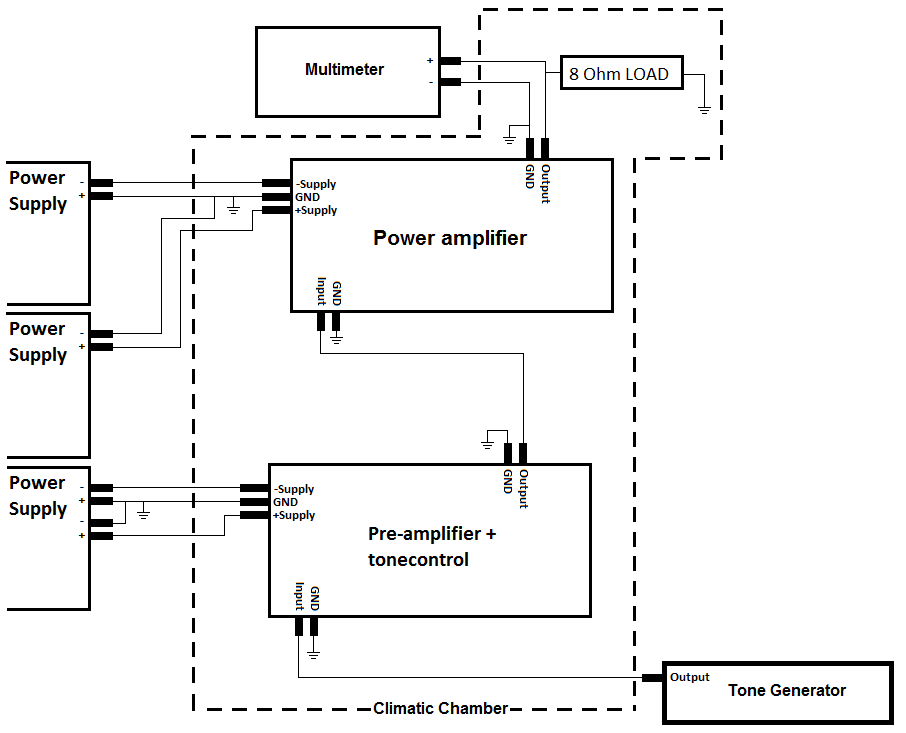
\includegraphics[scale=.8]{figures/filename}
	\flushleft 
	\caption{CAPTION\fxnote{Remember source}}
	\label{LABEL}
	\flushleft
	\textit{SOURCE}
\end{figure}

%--------- NOTES ------------------------------------------------------
%Fxnotes wont compile properly inside the figure, only in the caption.
%Filetype can be specified but isn't needed.

\noindent
\figref{LABEL}\\

\noindent
\Figref{LABEL}

\vspace{.5cm}
%Do not use \vspace{length} or \hspace{length} unless exceedingly necessary.

%--------- BIBLIOGRAPHY REF EKSAMPLE -----------------------------------
This reference only represents this line since it is before the punctuation mark\cite{YDing}. This next reference however represents the entire section. That is all of the preceding sentences in the entire section. This is due to the fact that it is now after the punctuation mark in the end of the section (this is not used in the middle of a section!).\cite{YDing}
%>>>>>>>>>>>>>>>PLEASE ALSO READ THE NOTE IN myBib.bib<<<<<<<<<<<<<<<<<<
\pagebreak	%||||||||
%	\section{Table Sample}

\begin{table}[H]
\caption{This Is a Table\label{LABEL}}
\begin{tabular}{|l|p{5cm}|l|l|l|}
  \hline
  \textbf{No.}&\textbf{Description}&\textbf{Min}&\textbf{Max}&\textbf{Requirements}\\
  \hline
  1 & Some Text & Some Text & Some Text & Some Text\\
    &           &           &           & Some More Text\\
    &           &           &           & Text Text\\
    &           &           &           & Text Text Text\\
  \hline
  2 & Some Text & Some Text & Some Text & Some Text\\
  \hline
  3 & 	By specifying the width of a column (|p\{5cm\}|) the cells
  		in that column will will not exceed	the specified width    %Enter is used only for clarity and will not affect the compiled output.
  		but instead expand downward.
  		
  		        & Some Text & Some Text & Some Text\\
  \hline
  4 & Some Text & Some Text & Some Text & Some Text\\
  \hline
  \multicolumn{2}{|l|}{Some Text} 	&	\multicolumn{3}{l|}{Some Text}\\
  \hline
  \multicolumn{2}{|l|}{Text Text} 	&	\multicolumn{3}{l|}{Text = Text}\\
  \multicolumn{2}{|l|}{}			&	\multicolumn{3}{l|}{Text = Text}\\
  \multicolumn{2}{|l|}{}			&	\multicolumn{3}{l|}{Text = Text}\\
  \multicolumn{2}{|l|}{}			&	\multicolumn{3}{l|}{Text = Text}\\
  \multicolumn{2}{|l|}{}			&	\multicolumn{3}{l|}{Text = Text}\\
  \hline
  \multicolumn{2}{|l|}{Some Text} 	&	\multicolumn{3}{l|}{Teeeexxtt}\\
  \multicolumn{2}{|l|}{}			&	\multicolumn{3}{l|}{\LaTeX}\\
  \hline      
\end{tabular}
\end{table}

\noindent
\tabref{LABEL}\\

\noindent
\Tabref{LABEL}

\pagebreak	%||||||||
%	\section{Equation Sample}

Ohms Law:
\begin{flalign}
  U &= I \times R \unit{\volt}
  \label{eq1}
\end{flalign}
%
Some explanation:
\begin{flalign}
  [Equation] &= [Number] \unit{Unit}
  \label{eq2}
\end{flalign}
%
Some explanation:
\begin{flalign}
  [Equation] &= [Number] \unit{Unit}
  \label{eq3}
\end{flalign}
%
Some explanation:
\begin{flalign}
  [Equation] &= [Number] \unit{Unit}
  \label{eq4}
\end{flalign}
%
Some explanation:
\begin{flalign}
  [Short Equation] &= [Number] \unit{Unit}
  \label{eq5}\\ %<-------------------------------------------------| Remember linebreak AFTER
  [Somewhat Longer Equation] &= [Number] \unit{Unit} %             | label when writing multiple
  \label{eq6}\\ %<-------------------------------------------------| equations.
  [Somewhat Quite a Lot Longer Equation] &= [Number] \unit{Unit}
  \label{eq7}
\end{flalign}
%
%
\eqref{eq1}\\
%
\eqrefTwo{eq1}{eq2}\\
%
\eqrefThree{eq1}{eq2}{eq3}\\
%
\eqrefFour{eq1}{eq2}{eq3}{eq4}\\
%
\eqrefFive{eq1}{eq2}{eq3}{eq4}{eq5}\\
%
\eqrefSix{eq1}{eq2}{eq3}{eq4}{eq5}{eq6}\\
%
\eqrefSeven{eq1}{eq2}{eq3}{eq4}{eq5}{eq6}{eq7}\\
%
\Eqref{eq1}\\
%
\EqrefTwo{eq1}{eq2}\\
%
\EqrefThree{eq1}{eq2}{eq3}\\
%
\EqrefFour{eq1}{eq2}{eq3}{eq4}\\
%
\EqrefFive{eq1}{eq2}{eq3}{eq4}{eq5}\\
%
\EqrefSix{eq1}{eq2}{eq3}{eq4}{eq5}{eq6}\\
%
\EqrefSeven{eq1}{eq2}{eq3}{eq4}{eq5}{eq6}{eq7}
%
\pagebreak	%||||||||
%|||||||												 ||||||||
%||||||||||||||||||||||||||||||||||||||||||||||||||||||||||||||||
%||||||||||||||||||||||||||||||||||||||||||||||||||||||||||||||||


%implementing front page:
\clearpage
\thispagestyle{empty}

\begin{figure}[H]
	\raggedleft
		
\includegraphics[width=0.2\textwidth]{figures/aaulogo-da.png}
\end{figure} 
\vspace*{\fill} 
\begin{center}	
\begin{Huge}
\textbf{Prædiktiv model til kapacitetsudnyttelse}\\
\vspace{5 mm}
P$5$ Semestersprojekt - Efteråret $2016$\\
\vspace{3 mm}
\end{Huge}
{\Large Gruppe $5405$}
\end{center}
\vspace*{\fill}

\begin{center}
\line(1,0){400}
\end{center}


%clears one or two pages to make the document start on right hand side:
%\cleardoublepage

%numbers the pages with Roman numeral - starts from "i":
\frontmatter

%implementing title sheet:
%\begin{document} 
\thispagestyle{empty}
%\begin{titlepage}
\begin{nopagebreak}
	{\samepage 
		
		\begin{tabular}{r}
			\parbox{\textwidth}{  \raisebox{11mm}{
\includegraphics[height=2cm]{figures/aaulogo-da.png}}
				\hfill \hspace{2cm} \parbox{8cm}{\begin{tabular}{l} %4.90
						{\small \textbf{\textcolor{MidnightBlue}{{$5$. Semester}}}}\\
						{\small \textbf{\textcolor{MidnightBlue}{School of Medicine and Health}}}\\
						%{\small \textbf{\textcolor{MidnightBlue}{}}}\\ 
						{\small \textbf{\textcolor{MidnightBlue}{Sundhedsteknologi}}}\\
						{\small \textcolor{NavyBlue}{Fredrik Bajers Vej $7$A}} \\
						{\small \textcolor{NavyBlue}{$9220$ Aalborg}} \\
						%{\small \textcolor{NavyBlue}{\emph{http://www.smh.aau.dk/}}}
			\end{tabular}}}
		\end{tabular}
		
		\begin{tabular}{cc}
			\parbox{7cm}{
				\begin{description}

%\item {Titel:}
%
%Prædiktiv model til kapacitetsudnyttelse\\

\item {Tema:} 

\small{
Klinisk teknologi
}

\end{description}

\parbox{8cm}{

\begin{description}
\item {Projektperiode:}\\
   P$5$, Efteråret $2016$\\
   
\item {Projektgruppe:}\\
  $5405$\\
  
\item {Medvirkende:}\\
Linette Helena Poulsen\\
Maria Kaalund Kroustrup\\
Nirusha Jeevanadan \\
Rolf Oberlin Hansen\\
Sageevan Sayananthan \\
Sebastian Munk \\

\hspace{2cm}
\item {Vejleder:}\\
Hovedevejleder: Pia B. Elberg \\
Kliniske vejleder: Sten Rasmussen \\
Klinisk bivejleder: Christian Kruse. \\  
\end{description}

}
\begin{description}
\item {Sider: XX}
\item {Appendikser: XX}
\item {Afsluttet:}
\end{description}
\vfill } &
\parbox{7cm}{
  \vspace{.15cm}
  \hfill 
  \begin{tabular}{l}
  {Synopsis:}\bigskip \\
  \fbox{
    \parbox{6.5cm}{\bigskip
     {\vfill{\small Overlæge Sten Rasmussen udtaler, at omfanget af kapacitetsmangel på ortopædkirurgisk afdeling på Aalborg Universitetshospital opleves stigende og tiltagende. Hertil forekommer der i år $2017$ en ny budgetaftale, der omhandler hurtigere udredning. Dette forventes at kunne skabe udfordringer for patientplanlægningen og kapacitetsudnyttelsen. Ubalance i kapacitetsudnyttelsen kan medvirke til komplikationer ift. arbejdsvilkår og patientsikkerhed. Herved kan en effektivisering af planlægningen medvirke til at opretholde en balance i kapacitetsudnyttelsen. En mulig løsning til dette kan være anvendelse af prædiktiv modellering til estimering af elektive patienters indlæggelsesvarighed. Det kan konkluderes, at en prædiktiv model kan anvendes til at estimere indlæggelsesvarigheden. Det er på baggrund af denne projektrapport ikke muligt at vurdere præcisionen af denne model, hvorfor yderligere studier er påkrævet.
     \bigskip}}
     }}
   \end{tabular}}
\end{tabular}} \vspace{1.3cm}
\raggedleft
\textit{\tiny Offentliggørelse af rapportens indhold, med kildeangivelse, må kun ske efter aftale med forfatterne.}\nopagebreak
\\
\end{nopagebreak}
%\end{titlepage}
%\end{document}
 %	\cleardoublepage

% FORORD OG LÆSEVEJLEDNING
%\chapter*{Forord og læsevejledning}

\section*{Forord}
Dette projekt er udarbejdet af gruppe $16$gr$5405$, $5$. semesters studerende på ingeniøruddannelsen sundhedsteknologi på Aalborg Universitet. Projektet er udarbejdet i perioden $2$. september til $19$. december år $2016$. Projektforslaget er stillet af Sten Rasmussen, overlæge på ortopædkirurgisk afdeling på Aalborg Universitetshospital, og omhandler prædiktiv modellering til forudsigelse af indlæggelsesvarigheden for patienter mhp. at effektivisere planlægningen. 


Vi vil gerne takke hovedevejleder Pia B. Elberg, kliniske vejleder Sten Rasmussen samt kliniske bi-vejleder Christian Kruse for vejledning og feedback gennem hele projektperioden. Derudover vil vi give en særlig tak til ortopædkirurgisk afdeling på Aalborg Universitetshospital for samarbejdet. 


\section*{Læsevejledning}
Rapporten er inddelt i fem kapitler. Det første kapitel indeholder projektets indledning samt den initierende problemstilling, der ligger til grund for problemanalysen, som fremgår af andet kapitel. Metoden beskrives i tredje kapitel. Fjerde kapitel analyserer implementeringen af en prædiktiv model på ortopædkirurgisk afdeling ift. forudsigelse af indlæggelsesvarighed for patienter mhp. planlægning af disse. Det fjerde kapitel er syntese, der indeholder en diskussion, konklusion samt perspektivering af projektet. Kapitlerne efterfølges af bibliografi samt bilag. 


Til håndtering af kilder anvendes Vancouver-metoden. De anvendte kilder nummereres i kantede parenteser. Er referencen placeret efter et punktum i en sætning, tilhører den hele afsnittet. Er referencen placeret før et punktum, tilhører den sætningen. Er der placeret flere referencer efter hinanden, betyder dette, at der er anvendt flere referencer til den pågældende sætning eller afsnit. Referencer til bilag er ligeledes indsat i kantede parenteser og er placeret efter samme metode som kilder. 

Forkortelser er skrevet ud ved første anvendelse, hvorefter forkortelsen er skrevet i parentes. Denne forkortelse anvendes herefter fremadrettet i rapporten. 


Rapporten er udarbejdet i \LaTeX, herudover anvendes MATLAB $2016$b til databehandling samt visualisering af grafer. 
 \cleardoublepage

%the '*' allows the tableofcontents be excepted from the actual table of contents.
\tableofcontents*
%\cleardoublepage

%numbers the pages with Arabic numeral - starts from 1.
\mainmatter

%---------------------------INPUTS-------------------------------


% INDLEDNING
\chapter*{Forord og læsevejledning}

\section*{Forord}
Dette projekt er udarbejdet af gruppe $16$gr$5405$, $5$. semesters studerende på ingeniøruddannelsen sundhedsteknologi på Aalborg Universitet. Projektet er udarbejdet i perioden $2$. september til $19$. december år $2016$. Projektforslaget er stillet af Sten Rasmussen, overlæge på ortopædkirurgisk afdeling på Aalborg Universitetshospital, og omhandler prædiktiv modellering til forudsigelse af indlæggelsesvarigheden for patienter mhp. at effektivisere planlægningen. 


Vi vil gerne takke hovedevejleder Pia B. Elberg, kliniske vejleder Sten Rasmussen samt kliniske bi-vejleder Christian Kruse for vejledning og feedback gennem hele projektperioden. Derudover vil vi give en særlig tak til ortopædkirurgisk afdeling på Aalborg Universitetshospital for samarbejdet. 


\section*{Læsevejledning}
Rapporten er inddelt i fem kapitler. Det første kapitel indeholder projektets indledning samt den initierende problemstilling, der ligger til grund for problemanalysen, som fremgår af andet kapitel. Metoden beskrives i tredje kapitel. Fjerde kapitel analyserer implementeringen af en prædiktiv model på ortopædkirurgisk afdeling ift. forudsigelse af indlæggelsesvarighed for patienter mhp. planlægning af disse. Det fjerde kapitel er syntese, der indeholder en diskussion, konklusion samt perspektivering af projektet. Kapitlerne efterfølges af bibliografi samt bilag. 


Til håndtering af kilder anvendes Vancouver-metoden. De anvendte kilder nummereres i kantede parenteser. Er referencen placeret efter et punktum i en sætning, tilhører den hele afsnittet. Er referencen placeret før et punktum, tilhører den sætningen. Er der placeret flere referencer efter hinanden, betyder dette, at der er anvendt flere referencer til den pågældende sætning eller afsnit. Referencer til bilag er ligeledes indsat i kantede parenteser og er placeret efter samme metode som kilder. 

Forkortelser er skrevet ud ved første anvendelse, hvorefter forkortelsen er skrevet i parentes. Denne forkortelse anvendes herefter fremadrettet i rapporten. 


Rapporten er udarbejdet i \LaTeX, herudover anvendes MATLAB $2016$b til databehandling samt visualisering af grafer. 

\chapter{Metode}
%Dette projekt er udarbejdet mhp. at kunne analysere en prædiktiv model, der har til formål at forudsige indlæggelsesvarigheden for patienter på OA. For at belyse den initierende problemstilling, undersøges det i problemanalysen, hvordan afdelingen påvirkes af ubalance i kapacitetsudnyttelsen samt, hvilken betydning handleplanen 2017 vil have for afdelingen. Denne problemanalyse leder frem til en problemformulering, der herefter leder frem til en analyse af prædiktiv modellering. Dette vurderes ud fra en analyse af implementeringen samt betydningen af en prædiktiv model. Herefter vil problemanalysen, problemformuleringen samt analysen af prædiktiv model diskuteres, konkluderes og perspektiveres i en syntese. 

Dette kapitel omhandler metode anvendt i projektrapporten. Projektet tager udgangspunkt i litteratur samt interviews af personale fra afdelingen, statistik og data fra OA. 


\section{Litteratursøgning}
For at kunne effektivisere litteratursøgningen for projektet er der opstillet kriterier. Disse er bl.a. at litteratur skal være den nyeste udgave af skriften, at kilder som udgangspunkt ikke må være ældre end $20$ år og at der er et tilgængeligt DOI eller ISBN nummer. 
Det er så vidt muligt forsøgt at anvende peer-reviewede artikler, der eksempelvis er fundet gennem primo, NCBI eller SpringerLink. Herudover anvendes PRI, sundhedsdatastyrelsen, samt informationspjecer fra OA, da der primært søges litteratur for det danske sundhedssystem med fokus på OA. Der er dog anvendt litteratur fra andre lande, primært tværnationale europæiske studier, hvor der hertil er taget forbehold for forskelle i sundhedsvæsner.


\section{Interview}
Der er foretaget kvalitative interviews af to sygeplejersker samt én lægesekretær fra OA for at besvare tvivlsspørgsmål omkring kapacitet, arbejdsgang samt planlægning af patienter. Interviewene er afholdt, da nogle spørgsmål ikke har været mulige at besvare gennem litteraturen. Der er forinden interviewene udarbejdet spørgsmål for således at sikre, at de uklare spørgsmål blev besvaret. Disse spørgsmål fremgår af bilag[\ref{bilagA}]. Der blev ligeledes opstillet nogle kriterier for interviews. Herunder ønskes det at afholde mindst tre interviews med personale fra OA for at undersøge, hvorvidt der er overensstemmelse mellem svarene. Det ønskes, at personalet har arbejdet på OA i mindst ét år for at sikre, at de har kendskab til planlægningen og arbejdsgangen på afdelingen. Herudover ønskes det ikke, at personalet kender spørgsmålene på forhånd, for således at undgå bias i besvarelsen. Det foretrækkes at have en åben dialog, da det hermed er muligt at stille opfølgende spørgsmål for at sikre forståelse under interviewene. Efterfølgende er interviewene blevet transskriberet, hvilket fremgår af bilag \ref{bilagO1}, bilag \ref{bilagO2} og bilag \ref{bilagsek}.


\section{Behandling af data}
Der er i et tidligere projekt indsamlet data fra $970$ hospitalsindlæggelser på OA. Dette er indsamlet fra Clinical Suite i perioden fra juli til og med oktober år $2014$. Datasættet indeholder forskellige parametre for patienterne. Disse er fordelt over $78$ parametre, herunder demografiske- og kliniske faktorer. De $78$ parametre er dog ikke udfyldt for hver enkelt patient, hvilket resulterer i flere tomme celler. Hermed er datasættet behandlet for dette i MATLAB $2016$b, hvor udvalgte kolonner er samlet i et nyt subsæt, hvorefter rækker med tomme celler er fjernet. Denne databehandling har medført, at data opsamlet fra $970$ hospitalsindlæggelser er reduceret til $472$. I rapporten anvendes datasættet med $472$ hospitalsindlæggelser på OA til udarbejdelse af grafer i MATLAB, medmindre andet er angivet.
\chapter{Indledning}


Flere danske hospitalsafdelinger oplever i perioder at have flere patienter end der er kapacitet til, i form af mangel på sengepladser, personale eller rum\cite{Company2013}. Overskridelsen af kapaciteten resulterer bl.a. i, at personalet får mindre tid pr. indlagt patient, hvilket kan medføre gener for både personalet og patienter.\cite{Kjeldsen2015} I budgetfordelingen for Aalborg Universitetshospital i år 2017 indgår det, at ventetiden på en operation for elektive patienter skal reduceres fra 57 dage til 50 dage\cite{Budget2016}. Dette forventes at medføre, at det daglige antal elektive patienter, der indlægges, vil skabe en reducering i antallet af ledige sengepladser til akutte patienter. 

Et estimat fra 2016 indikerer, at procentdelen af danskere over 65 år vil stige fra $29~\%$ til $34~\%$ og dermed også antallet af patienter\cite{RegionNord2016}. En stigning i antallet af patienter vil i takt med kortere ventetid på behandling skabe et aktuelt problem ift. planlægning af indlæggelser samt kapacitetudnyttelse på ortopædkirurgisk afdeling. Ifølge en undersøgelse fra Dansk Sygeplejeråd, mener hver anden regionalt ansat sygeplejerske på tværs af regionerne, at den travle arbejdsdag påvirker patientsikkerheden\cite{Kjeldsen2015}. Foruden personalets øgede risiko for at begå fejl ift. behandlingen af patienter, kan der ligeledes opstå en sundhedsrisiko ved kapacitetsmangel. Manglen på fysisk kapacitet kan give anledning til at overflytte patienter til uhensigtsmæssige områder som f.eks. hosptialsgange\cite{Madsen2014}. Dermed er der opstået et aktuelt problem som vedrører kapacitetsmangel, og konsekvenserne af dette problem bør undersøges nærmere. Ved at udnytte kapaciteten på afdelingen opnås der mere sundhed for pengene\cite{Company2013}. På baggrund af dette opstilles følgende initierende problem:

\textit{Hvordan påvirkes ortopædkirurgisk afdeling på Aalborg Universitetshospital af ændringerne vedrørende kapacitetsudnyttelse og hvor udbredte er belægningsrelaterede problemer på afdelingen?}





% Der er i dag overbelægning på flere afdelinger på de danske hospitaler, hvoraf nogle afdelingerne berøres i hele og flere måneder ad gangen. \cite{2015} Overbelægning resulterer i, at sundhedspersonalet får mindre tid pr. indlagt patient. Ifølge en undersøgelse fra Dansk Sygeplejeråd, mener hver anden regionalt ansat sygeplejerske på tværs af regionerne, at den travle arbejdsdag går ud over patienternes sikkerhed \cite{Kjeldsen2015}. Et studie påviser, at ved blot én ekstra indlagt patient pr. sygeplejerske øges mortalitetsraten med $7~\%$ indenfor en indlæggelse på 30 dage \fxnote{Har stadig lidt svært ved om man kan forstå sætningen på den rigtige måde.} \cite{Aiken2014}. 

% Foruden sundhedspersonalets øgede risiko for at begå fejl ift. behandlingen af patienter, er der ligeledes en sikkerhedsrisiko forbundet ved overbelægning på hospitalerne. De ekstra patienter, der ligger på stuerne, gangene og vaskerummene, pga. overbelægning, er en større udfordring ved evakuering under brand. Pladsmangel, som medfører, at patienterne opholder sig i vaskerummene og på gangene, bevirker desuden til, at patienterne oplever et skærpet privatliv. \cite{Madsen2014}

% Aalborg universitetshospital har i et tidligere projekt indsamlet data fra $1.000$ hospitalsindlæggelser. Disse data inkluderer blodprøveanalyser og knoglescanninger (DXA), hvilket formodes at kunne anvendes til udvikling af en prædiktiv model, der kan estimere indlæggelsesvarigheden blandt patienter. Denne rapport vil på baggrund af dette undersøge, hvorvidt det er muligt at forudsige indlæggelsesvarigheden ved brug af machine learning. \fxnote{mangler stadig noget om begrundelsen for valg af machine learning}



% \section{Initierende problemstilling} \fxnote{Dette er ikke den endelige problemstilling}
% Hvordan påvirkes personalet og patienterne af overbelægning på hospitaler, og hvilke konsekvenser har overbelægning i forhold til sikkerheden på afdelingerne?
% Hvilke typer af machine learning findes der, samt hvor benyttes det i dag?




% PROBLEMANALYSE
\chapter{Problemanalyse}
\section{Kapacitet} \label{kap}
% Skriv ift kapacitet (ift sengepladser, persona - hvilken betydning har hhv. 95 \% kapacitet mod 105 \%)
Kapacitetudnyttelse betegner forholdet mellem aktivitet og kapacitet. Aktivitet omhandler patient og kontakt, herunder består kontakt af forundersøgelse, behandling og kontrol. Kapacitet omfatter antallet af personale, udstyr og rum, hvor personalet består af læger, sygeplejersker og sekretærer. Udstyret beskriver antallet af maskiner på en afdeling og antallet af rum beskriver opbevarelsen af udstyret. Den samlede kapacitetsudnyttelse er defineret ud fra, at der produceres mest muligt for de investerede ressourcer.\cite{Company2013} 

\begin{figure}[H]
	\flushleft 
	\centering
	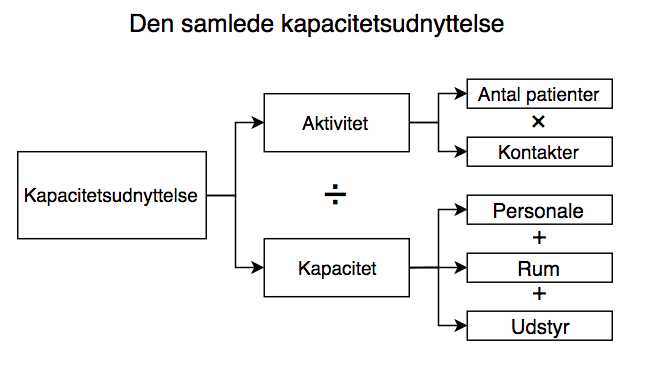
\includegraphics[scale=.65]{figures/Kapacitetsudnyttelse.png}
	\flushleft
	\caption{\textit{Den samlede kapacitetsudnyttelse som er definineret ved forholdet mellem aktivitet og kapacitet. Aktivitet omfatter antallet af patienter samt kontakter og kapacitet omfatter personale, rum og udstyr.}\cite{Company2013}}
	\label{kapacitet}
\end{figure}

\noindent
Ud fra \figref{kapacitet} fremgår det, at kapacitetsudnyttelse er forholdet mellem aktivitet og kapacitet. Dertil ses aktivitet som antal patienter multipliceret med kontakter. Kapaciteten udgør personale, rum og udstyr lagt sammen. Antallet af patienter, der repræsenterer en del af aktivitet beskriver ligeledes belægning på hospitalets afdelinger.\cite{Company2013} 

Belægning er defineret ud fra antallet af patienter, der er normeret til på en afdeling\cite{Heidmann2014}. Når en $100~\%$ belægning opnås, svarer dette til, at de disponible sengepladser på en afdeling er taget i brug. Ved en belægning på over $100~\%$ betyder det, at der er flere patienter end afdelingen er normeret til, hvilket vil sige, at afdelingen yder mere end der er kapacitet til. Ud fra \figref{kapacitet} vil dette betyde, at der ikke er ligevægt mellem aktivitet og kapacitet, hvilket i dette tilfælde vil forårsage kapacitetsmangel på afdelingen. Det kan derfor være nødvendigt, at personalet skal varetage flere patienter samt arbejdsopgaver, det kan ligeledes være nødvendigt at tilkalde ekstra personale for at opnå en balance i kapacitetsudnyttelsen.
Hvis der derimod er en belægning på under $100~\%$ er der omvendt færre patienter end afdelingen er normeret til. Dette betyder, at der er flere sengepladser end patienter, hvilket ligeledes fører til en ubalance i kapacitetsudnyttelsen. I denne situation er der mere personale end nødvendigt til at varetage de enkelte patienter, hvilket betyder, at der ikke er fuld udnyttelse af personalets arbejdskraft.\cite{Pauly1986} 

Det anses herved vigtigt, at der er balance mellem aktivitet og kapacitet, således de investerede ressourcer udnyttes optimalt. Det ønskes derfor at opnå en kapacitetsudnyttelse på $100~\%$. Ud fra dette vil der fremover undersøges betydningen af kapacitetsudnyttelse på ortopædkirurgisk afdeling på Aalborg Universitetshospital. 

\subsection{Ortopædkirurgisk afdeling}
Kapacitetsudnyttelse afhænger af det budget som hver afdeling har til rådighed. Dette budget udregner Sundhedsstyrrelsen ud fra diagnoserelaterede grupper (DRG). DRG anvendes til at analysere omkostninger og aktivitet på et hospital.\cite{DRG2016} Ortopædkirurgisk afdeling har et budget på $700.872.744$ kr, som svarer til 17,2 \% af det samlede budget for alle afdelinger på Aalborg Universitetshospital. Det samlede DRG for afdelingerne på Aalborg Universitetshospital er illusteret af \figref{DRG_budget}.\cite{Rasmussen2016}
Størstedelen af budgettet anvendes til personale- og patientudgifter, som svarer til hhv. 60 \% og 32 \%. Det resterende budget anvendes til bygninger, it, apparatur, inventar samt drift og service\cite{Noegletal2016}. 


\begin{figure}[H]
	\flushleft 
	\centering
	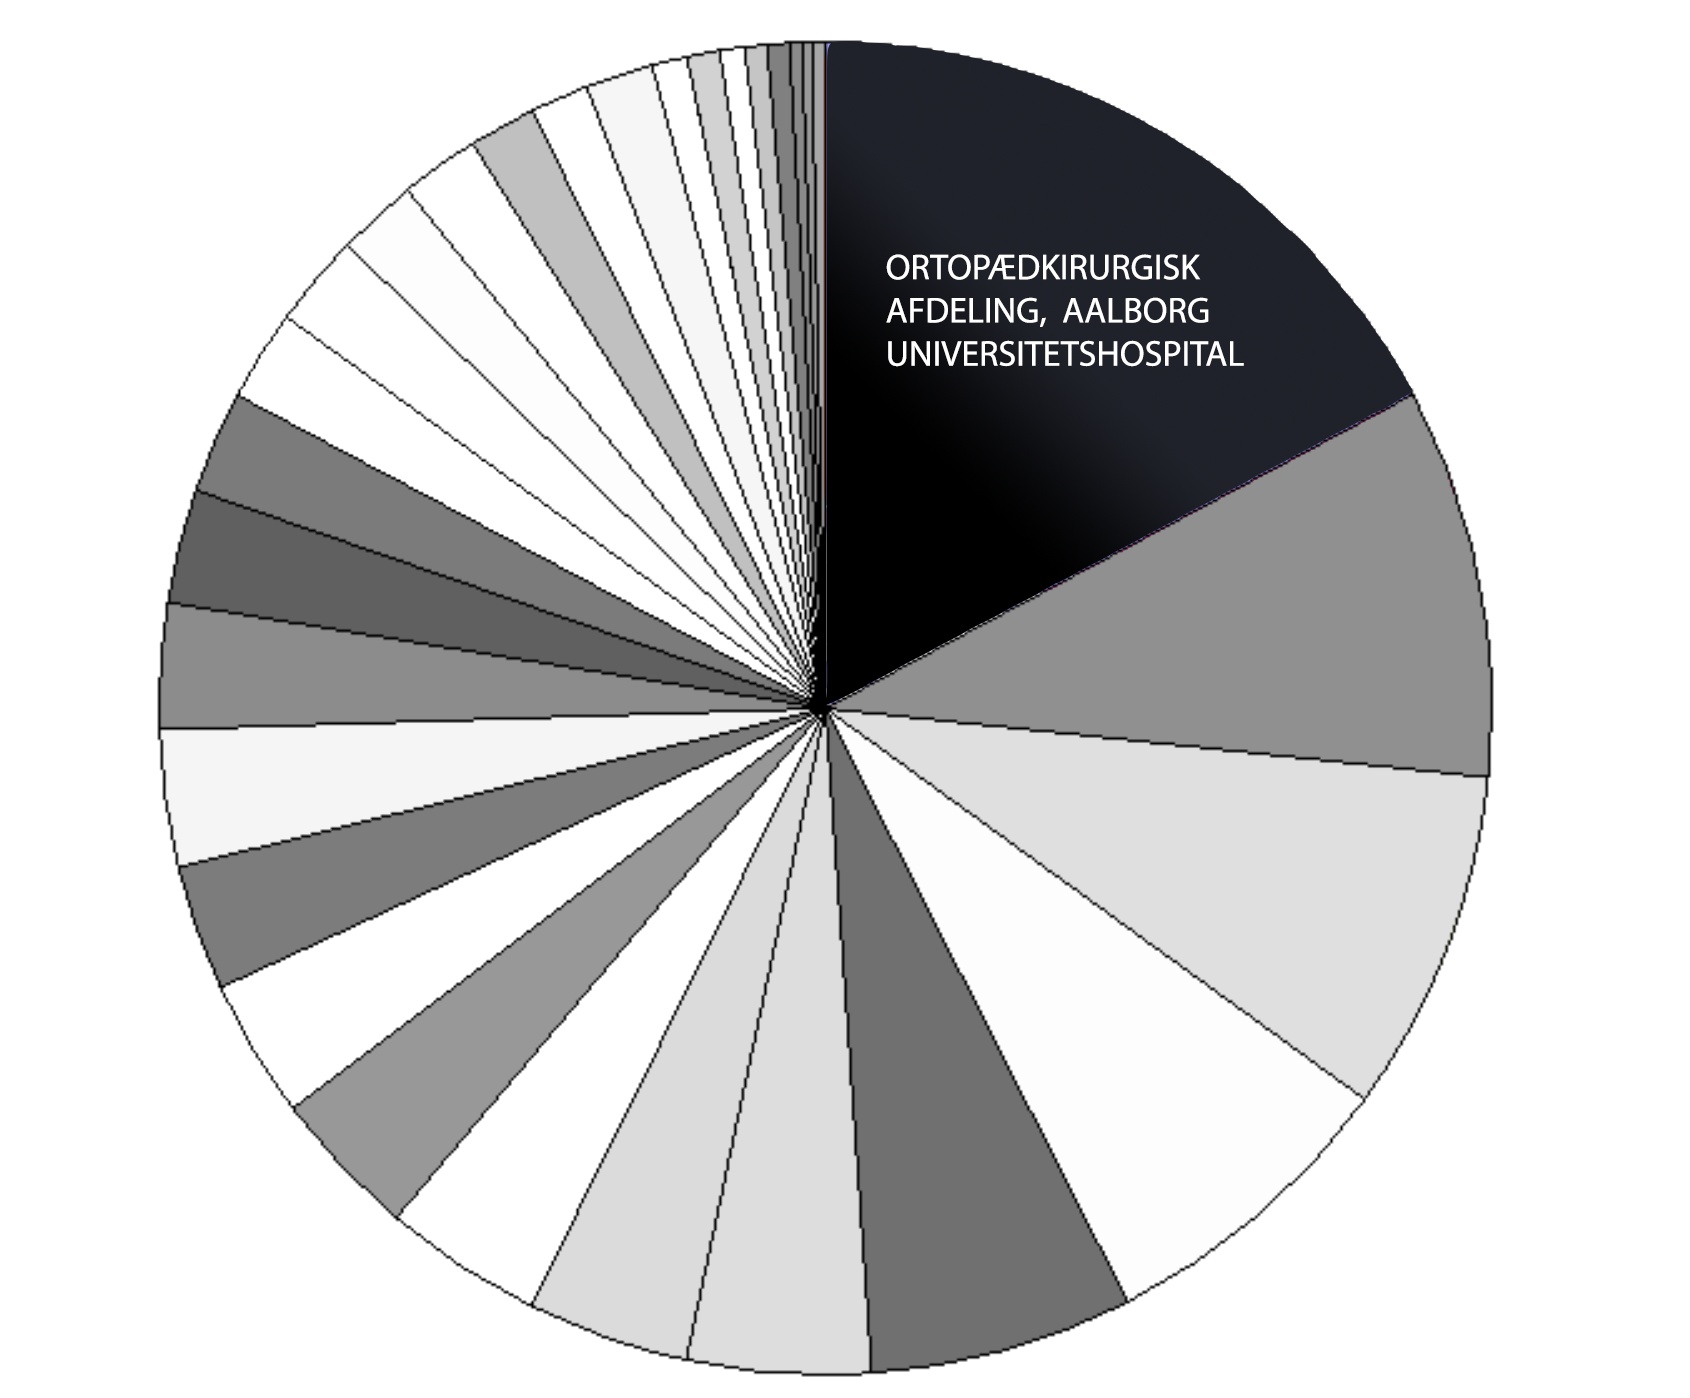
\includegraphics[scale=0.45]{figures/Ortopaeddiagram.png}
	\flushleft
	\caption{\textit{Fordeling af DRG for samtlige afdelinger på Aalborg Universitetshospital. Det fremgår, at ortopædkirurigisk afdeling har en større andel end de resterende afdelinger.}\cite{Rasmussen2016}}
	\label{DRG_budget}
\end{figure}


\subsubsection{Personalearbejde} 
% Hvordan opleves belægning generelt på OA på Aalborg UH? Hvordan varetages opgaver af personalet? Hvordan er vagtskifte? Hvor langt tid arbejdes der gennemsnitlig om dagen?
%Som beskrevet i \autoref{sec:kap} er personalet en del af kapacitet. Personalet ses som en væsentlig faktor for at udnytte kapaciteten effektivt. 
På ortopædkirurgisk afdeling på Aalborg Universitetshospital arbejder personalet i gennemsnit 37 timer om ugen\cite{Danske2015}. Vagterne kan variere fra XX til XX timer, hvoraf det både kan være nat- og dagvagter. Der er indlagt betalte pauser, hvilket betyder, at personalet skal være til rådighed under pausen. Pauserne er opdelt i XX om dagen. Afdelingen er delt op i XX vagthold og har vagtskifte hver XX time. Personalet varetager XX patienter om dagen. \fxnote{Vi mangler informationer for at kunne skrive dette færdigt.}

\subsubsection{Patientindlæggelse}
% Hvordan foregår indlæggelsen på OA på AUH? Hvornår indlæggelses patienterne (elektive patienter) og hvornår på dagen udskrives patienter (både elektive og akutte patienter) Hvor mange patienter hhv. akutte vs. elektive patienter? Hvad er deres buffer i forhold til elektive patienter, således der er plads til de akutte indlæggelser? indkaldes elektive patienter, hvis der er mindre akutte i en periode end der er estimeret til? Øges den normerede kapacitet under overbelægning ved at indkalde vikarbureau? (Altså tager man samme mængde elektive patienter ind.) 


Som beskrevet i afsnit \ref{kap} ønskes en $100~\%$ kapacitetsudnyttelse, dertil ønskes ligeledes en belægning på $100~\%$. 
For at opfylde dette skal der være ligevægt mellem antallet af sengepladser og patientindlæggelser. På ortopædkirurgisk afdeling har de XX sengepladser til rådighed, som er fordelt på XX afsnit.

Ortopædkirurgisk afdeling modtager både elektive samt akutte patienter. Elektive patienter omfatter både indlagte og ambulante patienter. Ved pludselig forværret tilstand kan elektive patienter skifte status fra elektiv til akut. Akutte patienter defineres som personer, der er henvist til hospitalet efter en akut opstået tilstand. Sammenlignes der med de resterende afdelinger på Aalborg Universitetshospital, har ortopædkirurgisk afdeling flest elektive indlæggelser.\cite{RegionNord2016} Elektive patienter indlægges i tidsrummet XX-XX og udskrives i tidsrummet XX-XX. Udskrivelsen af akutte patienter foregår i samme tidsrum. På afdelingen planlægges elektive patienter med forbehold for, at der er uforudsigelige indlæggelser af akutte patienter pr. XX. Herunder planlægges XX elektive patienter, således at der er plads til XX akutte patienter.\fxnote{Vi mangler informationer for at kunne skrive dette færdigt + tilføjelse af Sebastians grafer (elektive/akuttte) + (indlæggelse/udskrivelse)}
\section{Ubalance i kapacitetsudnyttelse}
Ved kapacitetsmangel på ortopædkirurgisk afdeling forekommer en omstrukturering af personalets arbejdsopgaver, som sikre patientens behov, opretholdelse af kvalitet og udnyttelse af kompetencer. Dette er med henblik på at opnå en balance mellem de ressourcer og de krav, der stilles i den pågældende situation.\cite{Bjerg2016}  %Generelt er personalet den begrænsende faktor for planlægning og kapacitetsudnyttelse\cite{Company2013}. 

\subsection{Arbejdsvilkår} \label{Per_sik}
%Hvordan påvirkes personalets arbejdsrutiner ved kapacitetsmangel? Hvor længes må deres arbejdsdag maksimalt være? Stiger antallet af fejl når personalet varetager en større arbejdsbyrde end planlagt? Hvor omkostningsfuldt er det? 

I tilfælde af kapacitetsmangel er der udarbejdet en arbejdstilrettelæggelse af Region Nordjylland for personalet på ortopædkirurgisk afdeling. Ved kapacitetsmangel påtager lederen, eller dennes stedfortræder, ansvaret for at finde en løsning på dette problem. Dette kan betyde, at det afgående vagthold skal blive indtil en midlertidig løsning er fundet eller en tidligere indkaldelse af det næste vagthold. I nogle tilfælde kan det være nødvendigt at låne ressourcer fra andre afsnit eller indkalde personale fra vikarbureauet. Derudover undersøges det, hvorvidt behandlingen af elektive patienter kan aflyses.\cite{Bjerg2016} 

Ved overarbejde må en arbejdsuge for en sygeplejerske, ifølge arbejdstidsaftalen indgået med Dansk Sygeplejeråd, ikke overstige 48 timer\cite{Danske2015}. \fxnote{Spørgsmål til sygeplejersker: Hvordan prioriteres pauser under overbelægning?} Hvis sundhedspersonalet er nødsaget til at arbejde længere end den normale arbejdstid, viser dette sig at have en negativ indvirkning på personalets arbejdesopgaver\cite{Dinges2004}. Overarbejde kan resultere i en presset arbejdsdag og dermed en forringet kvalitet af behandlingen\cite{Kjeldsen2015}. Dertil mener hver anden regionalt ansat sygeplejerske på tværs af regionerne, at den travle arbejdsdag påvirker patienternes sikkerhed\cite{Kjeldsen2015}.

%Den større patientbyrde, der skal varetages ved en belægning over 100\%, medvirker til en øget arbejdsbyrde for det tilstedeværende personale.\fxnote{Spørgsmål til sygeplejersker: Hvor mange patienter skal i under normale omstændigheder varetage? Og hvordan fungerer det under overbelægning? Fordeles de enkelte patienter mellem jer?} \cite{Dinges2004,Aiken2002,Madsen2014}
%Det er forsøgt at kapacitsoptimere, med en reduktion af sengepladser på $30~\%$ i perioden $1996$ til $2011$ \cite{Dinges2004,Aiken2002,Madsen2014} 


\subsection{Patientsikkerhed}
%Hvordan påvirker kapacitetsmangel ift. brandsikkerhed? Laver personalet flere fejl, som går ud over patienterne ved overbelægning? Hvordan fungerer omrokering af patienter (gangarealer, vaskerum ect.)? Hvor omkostningsfuldt er det for OA’s budget? brandsikkerhed og Genindlæggelse
Under perioder med kapacitetsmangel er det ofte nødvendigt at overflytte patienter til andre afdelinger, gangarealer eller fyldte stuer, herved er det ofte patienter, der snart udskrives, der overflyttes. \fxnote{Sygeplejersker: Vi vil gerne høre om der prioriteres i forhold til hvilke patienter der flyttes. Er der en bestemt afdeling i flytter patienterne over på eventuelt en afdeling der ligner ortopædkirurgisk?} Overflytningen kan belaste både fysiske og psykiske forhold for patienter såvel som pårørende\cite{Heidmann2014}. Herunder kan skærpet privatliv forekomme hos patienter, der er flyttet til gangarealer eller fyldte stuer\cite{Madsen2014}. 

Som nævnt i afsnit \ref{Per_sik} forringes kvaliteten af behandlingen ved overarbejde, dertil ses det ligeledes, at mortalitetsraten øges med $1,2~\%$ ved en overskridelse af belægningen med $10~\%$, ifølge et dansk studie fra år $2014$\cite{Madsen2014}. Hertil understreges det, at der kan være ukendte parametre, der påvirker mortalitetsraten, og det nødvendigvis ikke er belægning, der er den primære årsag til en øget mortalitet. For at undgå forringet kvalitet af behandling forsøges det at få patienterne udskrevet tidligere, således et ønske om balance mellem aktivitet og kapacitet opnås.

%\fxnote{Tidligere afsnit: Hvordan er fordelingen af elektive og akutte patinter? Kan elektive patienter tages ind før der er normalbelægning?} 

Der tilkaldes en brandvagt til afdelingen, hvis en belægning over $100~\%$ har fundet sted i over $4$ timer for således at sikre patienterne ved evakuering under brand. En brandvagt kan højest overvåge to afdelinger på samme etage, hvorfor det kan være nødvendigt, at der indkaldes flere. Det er afdelingens ansvar at afvikle belægningsproblemet og kapacitetsmanglen hurtigst muligt ved at udskrive patienter eller overflytte patienter til andre afdelinger. \fxnote{Har skal indsættes hvis de har et samarbejde med en anden afdeling} Hver gang der tilkaldes en brandvagt faktureres dette af Aalborg Universitetshospital.\cite{Beredskab2016}



\section{Omfang af belægning}
På ortopædkirurgisk afdeling på Aalborg Universitetshospital ses en varierende belægningsgrad fra måned til måned. Belægningsgraden er antallet af disponible senge i brug. På \figref{maxminbelaeg} ses den varierende belægning fra år $2014$ til $2015$ på ortopædkirurgisk afdeling. \cite{SDS2015}


\begin{figure}[H]
	\flushleft 
	\centering
	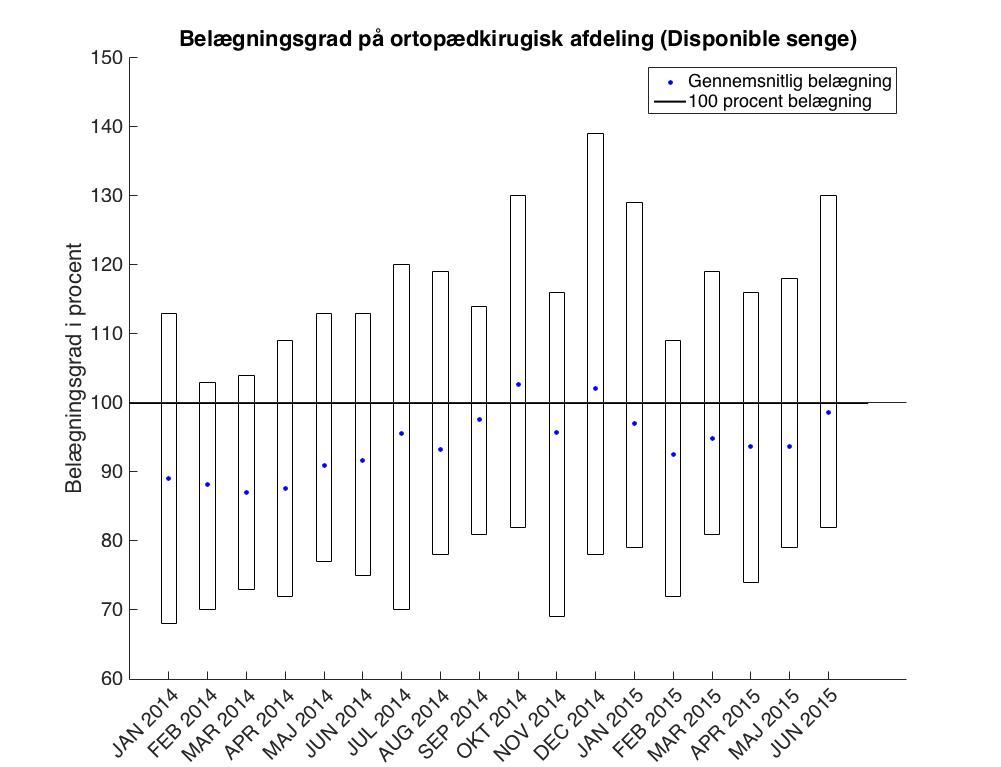
\includegraphics[scale=.45]{figures/maxminoverbelaeg.png}
	\label{maxminbelaeg}
	\flushleft
	\caption{\textit{Figuren illustrerer belægningsgraden over 18 måneder fra år $2014$ til $2015$ på ortopædkirurgisk afdeling på Aalborg Universitetshospital. Søjlerne viser belægning ift. $100\%$ belægning, dertil ses den gennemsnitlige belægning for hver måned som et punkt. \cite{SDS2015}}}
\end{figure}


Det fremgår af \figref{maxminbelaeg}, at ortopædkirurgisk afdeling oplever en belægning hhv. over og under én ønskede belægning på $100 \%$. I december måned år $2014$ ses en maksimal belægning på $1XX \%$ og en minimums belægning på $xx \%$. Dette indikerer, at ortopædkirurgisk afdeling oplever belægning over $100 \%$ i kortvarige perioder. Da \figref{maxminbelaeg} ikke viser belægningsperioden er det uvist om, hvorvidt belægningen over $100 \%$ opleves i timer eller flere dage. Der skal herudover tages forbehold for, at \figref{maxminbelaeg} både indeholder elektive samt akutte indlagte patienter, og derfor er uvist om, hvorvidt det er akutte patienter, der resulterer i en belægningsgrad på over $100 \%$. Der ses ligeledes en gennemsnitlig belægning pr. måned på \figref{maxminbelaeg}. Denne ses hyppigst under $100 \%$ belægning, hvortil der kun ses oktober samt december i år $2014$ med en gennemsnitlig belægning på over $100 \%$ belægning. Derved opleves der ikke en gennemsnitlig belægning på over $100 \%$ i $16$ ud af de $18$ oplyste måneder. \cite{SDS2015}


For at underbygge belægningsgraden yderligere, illustrerer \figref{antaldage} antal dage pr. måned med en belægningsgrad på over $100 \%$. Denne graf er udarbejdet ud fra ortopædkirurgisk afdeling over de samme 18 måneder fra år $2014$ til $2015$ som \figref{maxminbelaeg}. \cite{SDS2015} 

\begin{figure}[H]
	\flushleft 
	\centering
	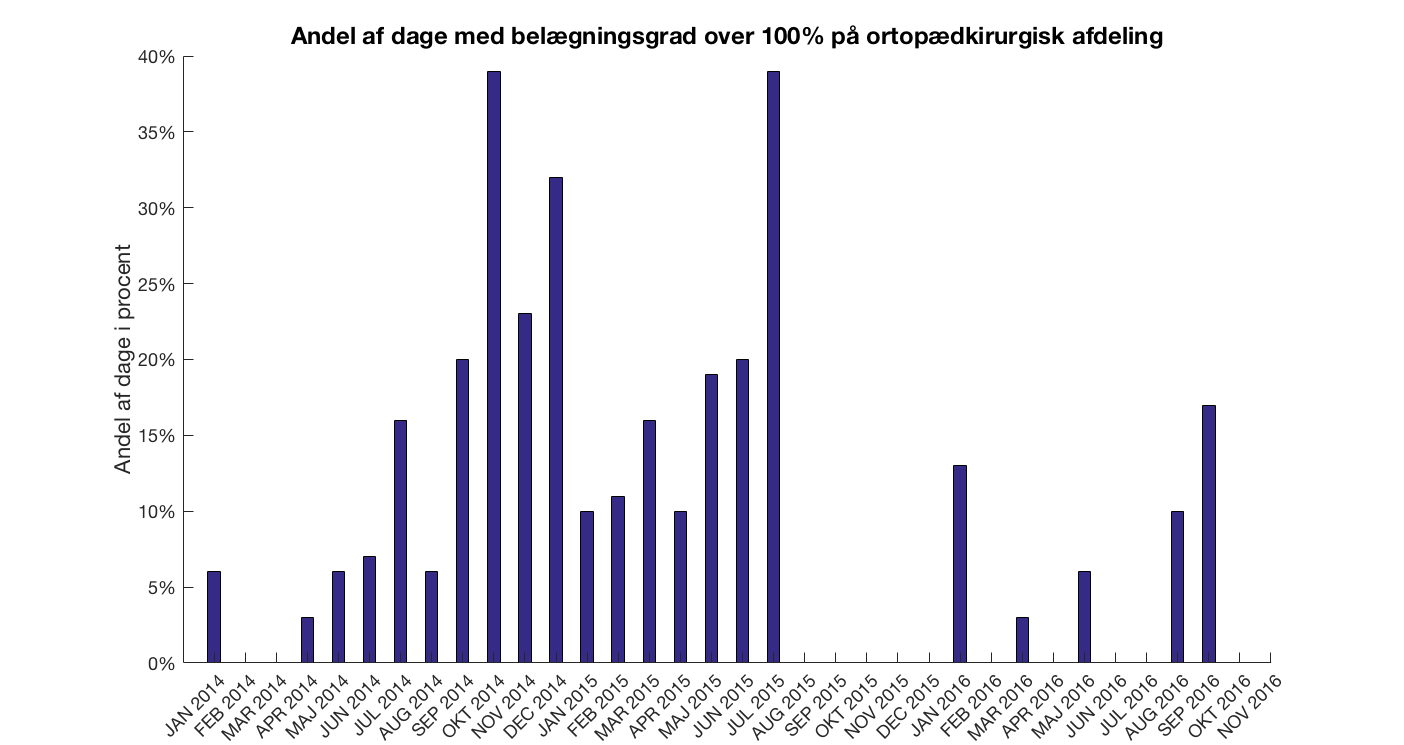
\includegraphics[scale=.7]{figures/antaldage.png}
	\label{antaldage}
	\flushleft
	\caption{\textit{Figuren illustrerer antal dage med en belægningsgrad over $100 \%$ fra januar 			$2014$ til juni $2015$ på ortopædkirugisk afdeling på Aalborg Universitetshospital. 					\cite{SDS2015}}}
\end{figure}


Af \figref{antaldage} ses det, at der i oktober måned år 2014 opleves en belægning på over $100 \%$ i 19 dage. Det vides dog ikke, hvorvidt der er tale om én ekstra eller flere patienter, der udgør en belægningsgrad på over $100 \%$, samt hvor længe patienterne er indlagt på afdelingen. Det ses i \figref{maxminbelaeg}, at der i oktober måned år 2014 opleves en belægning på $130 \%$, hvilket kan opholdes mod de 19 dage. Det skal understreges, at begge grafer er angivet i måneder, og det er derfor uvist om, hvor mange patienter, der er indlagt pr. dag. Derudover er figurerne, \figref{maxminbelaeg} og \figref{antaldage}, udarbejdet over 18 måneder, hvilket angiveligt ikke er en repræsentativ periode for at konkludere et reelt problem på afdelingen. Dertil vides det ikke om belægningsgraden over $100 \%$ opleves som værende et problem på ortopædkirurgisk afdeling på Aalborg Universitetshospital eller om det blot er et strukturerings problem. 
\section{Problemformulering}
\textit{Hvordan kan indlæggelsesvarigheden for patienter på ortopædkirurgisk afdeling på Aalborg Universitetshospital forudsiges med henblik på at opretholde en kapacitetsudnyttelse på 100 \%?}


% PROBLEMLØSNING
\chapter{Problemløsning}
På ortopædkirurgisk afdeling på Aalborg Universitetshospital ønskes der, på baggrund af afsnit \ref{kap}, en $100~\%$ kapacitetsudnyttelse med henblik på at udnytte de tilgængelige ressourcer optimalt. Kapacitetsudnyttelse er forholdet mellem aktivitet og kapacitet, hvoraf antal patienter er en betydende faktor ift. aktivitet. 
Det fremgår af afsnit \ref{omfang}, at belægningsgraden på ortopædkirurgisk afdelingen er varierende for hver måned. Ved en belægning over $100~\%$ vil afdelingen opleve kapacitetsmangel, hvilket vil medføre, at personalet skal yde mere end afdelingen har kapacitet til. Derimod vil afdelingen ved en belægning under $100~\%$ forårsage, at der ikke er fuld udnyttelse af personalets arbejdskraft. Derved oplever ortopædkirurgisk afdeling en ubalance i kapacitetsudnyttelsen. 
For at opnå en kapacitetsudnyttelse på $100~\%$, skal en ligevægt mellem aktivitet og kapacitet forekomme. Denne ligevægt kan tilnærmes ved at justere på én af faktorerene under aktivitet eller kapacitet\cite{Bames2015}. Det kan herunder forsøges at effektivere planlægningen af patienter og dertil forsøge at estimere indlæggelsesvarigheden for de indlagte patienter. 
På baggrund af dette opstilles følgende hypotese:\\

\noindent
\textit{Indlæggelsesvarigheden for patienter kan benyttes til at effektivisere kapacitetsudnyttelsen.} 

\section{Forudsigelse af indlæggelsesvarigheden}
For at forbedre kapacitetsudnyttelsen på ortopædkirurgisk afdelingen undersøges det, hvorvidt indlæggelsesvarigheden kan forudsiges.
%Det fremgår af AFSNIT\fxnote{ref til afsnit}, at ortopædkirugisk afdeling på Aalborg Universitetshospital ikke fastholder en kapacitetsudnyttelse på $100$\%.\fxnote{snak sammen med Linette og Maria} 
Aalborg Universitetshospital har i et tidligere projekt indsamlet data fra $970$ hospitalsindlæggelser fra ortopædkirurgisk afdeling. Datasættet er indsamlet gennem digitale patientjournaler i perioden 1. august til 31. oktober år 2014. Disse data er fordelt på 78 forskellige parametre. Flere af parametrene for patienterne er ukendte, hvorfor præprocessering af datasættet anses nødvendigt. Ud fra parametrene i datasættet vil indlæggelsesvarigheden forsøges estimeres. 
\section{Forudsigelse af indlæggelsesvarigheden}
Ved ortopædkirurgiske operationer er der flere parametre, der kan have indflydelse på indlæggelsesvarigheden. Dette kan eksempelvis være demografiske parametre såsom alder samt køn og kliniske parametre som blodprøver, blodtab og operationstype. Da der kan opstå komplikationer under en operationen, som kan have indflydelse på indlæggelsesvarigheden opdeles parametrene præ- og postoperativt.


\subsection{Præoperativt}
På ortopædkirurgisk afdeling estimeres indlæggelsesvarigheden ikke på nuværende tidspunkt, dog vurderes indlæggelsesforløbet ud fra personalets erfaringer. Ud fra informationspjecer fra ortopædkirurgisk afdeling på Aalborg Universitetshospital informeres om, hvilke faktorer der kan være under en operation. Disse kan angiveligt forlænge indlæggelsesvarigheden. 


\subsubsection{Livsstilsfaktorer}
Livsstilsfaktorer tyder på at have betydning for komplikationer under en operation. Lavt præoperativt funktionsniveau og muskeltab er ofte aldersbetinget, hvilket kan medføre komplikationer og lang indlæggelsesvarighed. Hvorimod patienter med højt funktionsniveau ofte har kortere indlæggelsesvarighed.\cite{Kehlet2001, Janssen2002} Af \figref{alderogindlaeggelse} fremgår patientens alder samt indlæggelsesvarighed i perioden 1. august til den 31. oktober år 2014.


\begin{figure}[H]
	%\flushleft 
	\centering
	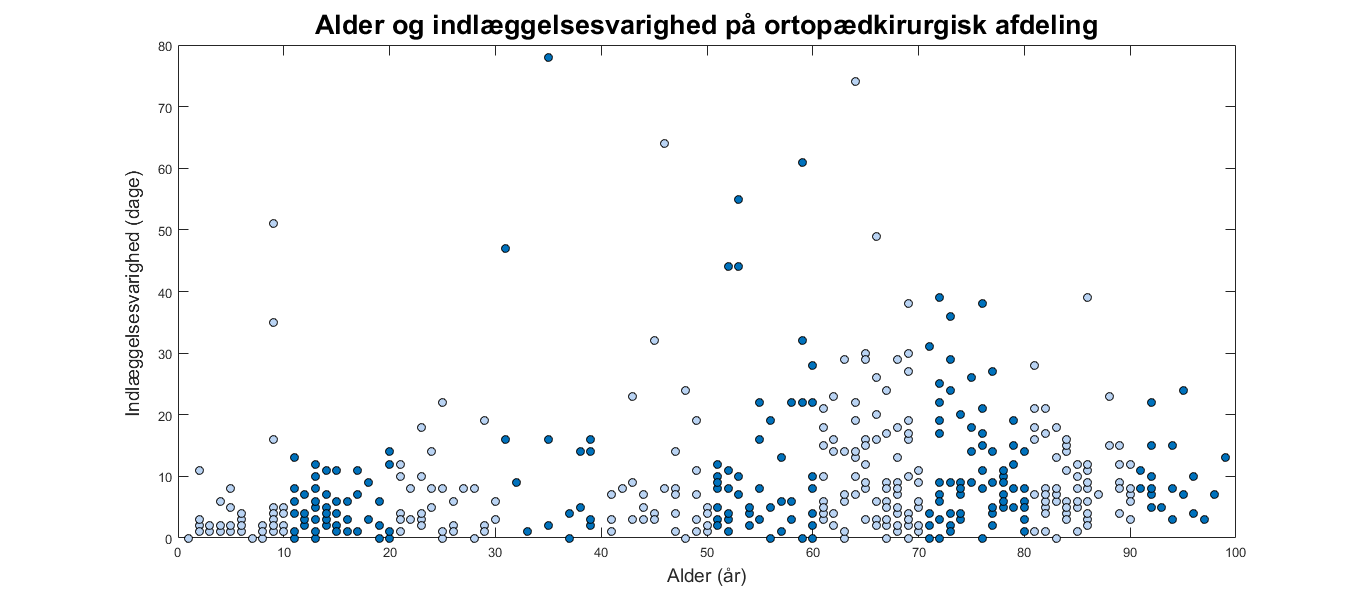
\includegraphics[scale=0.45]{figures/alderogindlaeg}
	%\flushleft
	\caption{\textit{Alder og indlæggelsesvarigheden for patienter på ortopædkirurgisk afdeling. Dette er over en periode på 3 måneder fra den 1. august til den 31. oktober år 2014.}}
	\label{alderogindlaeggelse}
\end{figure}


\noindent
På \figref{alderogindlaeggelse} fremgår det, at der er en bred aldersfordeling på ortopædkirurgisk afdeling. Derudover ses det, at indlæggelsesvarigheden for ældre patienter er mere varierende end yngre patienter, hvoraf denne spredning stiger med alderen. Det fremgår ligeledes, at de ældre patienter indlægges i længere tid end yngre patienter. Patienter under $30$ år er i gennemsnit indlagt 5 dage, hvor patienter over $30$ år i gennemsnit er indlagt 10,9 dage. Det er uvist om dette skyldes lavere funktionsniveau eller om der er andre faktorer der spiller ind, eksempelvis operationstype, som ældre hyppigere får foretaget, hvilket kan medvirke til den længere indlæggelsesvarighed.


Udover alder kan vægt ligeledes have en indflydelse på operationer foretaget på ortopædkirurgisk afdeling, da overvægt giver større risiko for blodpropper\cite{Ermonds2004}. Ved overvægt anbefales det derved at tabe sig før en eventuel operation. Foruden mindsket risiko ved opståen af komplikationer, kan smerter ligeledes reduceres ved vægttab.\cite{Nordjylland2014} På \figref{BMIogindlaeggelse} fremgår body mass index (BMI) samt indlæggelsesvarigheden i samme periode som \figref{alderogindlaeggelse}.

\begin{figure}[H]
	%\flushleft 
	\centering
	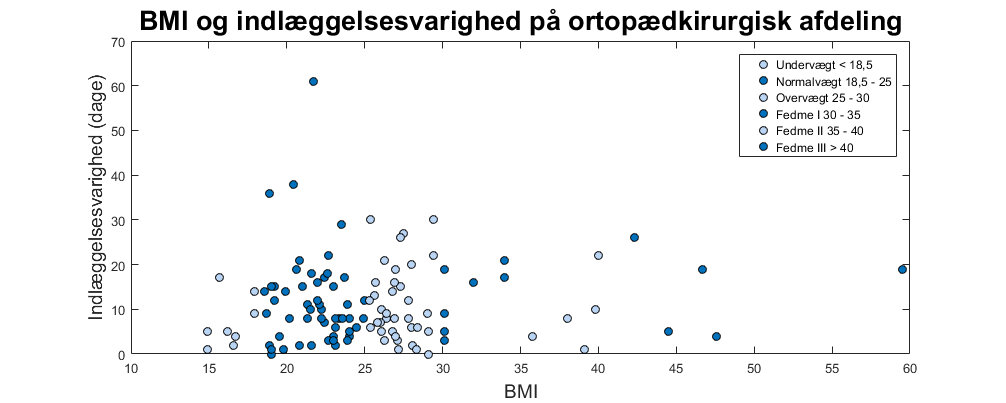
\includegraphics[scale=0.6]{figures/BMIogindlaeg}
	%\flushleft
	\caption{\textit{BMI og indlæggelsesvarigheden for patienter på ortopædkirurgisk afdeling. BMI er opdelt i 6 kategorier: Undervægtig, normalvægtig, overvægt fedme I, fedme II og fedme III. Dette er over en periode på 3 måneder fra den 1. august til den 31. oktober år 2014.}}
	\label{BMIogindlaeggelse}
\end{figure}


\noindent
Af \figref{BMIogindlaeggelse} fremgår det, at størstedelen af patienterne på ortopædkirurgisk afdeling befinder sig inden for vægtklassen, normal og overvægt. Indlæggelsesvarigheden er ligeledes mere varierende i disse klasser, hvor patienterne her er indlagt fra 0 til 61 dage. Indlæggelsesvarigheden er for patienter i normalvægt og overvægt klassen i gennemsnit 11,3, mens det for fedmeklasse I, II, III i gennemsnitlig 11,7 dage. Et højere BMI typer derfor ikke på, at have en betydning for en længere indlæggelsesvarighed. 


Andre livsstilsfaktorer såsom rygning og alkohol kan have betydning for komplikationer under operationer. Rygning kan være medvirkende til at knogler og sår heler langsommere. Ved operationer, hvor der skal transplanteres knoglevæv, f.eks. rygoperationer, afhænger operationens resultat af, at knoglevævet heler rigtigt. Definitionen af en ikke ryger er en person, der har været røgfri i op til 6 måneder, det anbefales derfor at stoppe med at ryge 6 måneder før den planlagte operation.\cite{Nordjylland2014} Fordelingen af ryger, tidligere ryger samt ikke ryger og, hvilken betydning dette har for indlæggelsesvarigheden fremgår af \figref{rygningogindlaeggelse}.


\begin{figure}[H]
	%\flushleft 
	\centering
	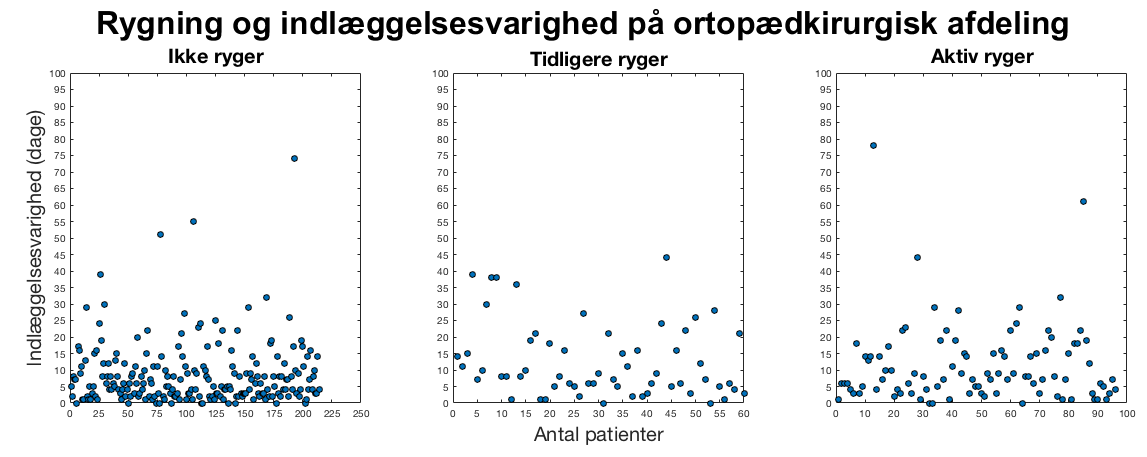
\includegraphics[scale=0.55]{figures/rygerogindlaeg}
	%\flushleft
	\caption{\textit{Rygning og indlæggelsesvarigheden for patienter på ortopædkirurgisk afdeling. Rygning er opdelt efter ikke ryger, eks-ryger og aktiv ryger. Eks-ryger defineres som røgfri i et halvt år. Dette er over en 3 måneders periode fra den 1. august til den 31. oktober år 2014.}}
	\label{rygningogindlaeggelse}
\end{figure}


\noindent
Det ses af \figref{rygningogindlaeggelse}, at størstedelen af ortopædkirurgisk afdeling ikke ryger. Derudover fremgår det, at variationen i indlæggelsesvarigheden er større for eks-rygere og rygere end for aktive rygere. Den gennemsnitlige indlæggelsesvarighed for ikke ryger er 8,4 dage, hvor den for eks-ryger og aktiv er henholdsvis 12,8 og 11 dage. Det tyder derfor på, at rygning har en betydning for indlæggelsesvarigheden.

Som tidligere nævnt kan alkohol ligeledes medføre øget risiko for komplikationer under operationer. Herunder kan der opstå øget blødning under operationer samt infektioner i såret.\cite{Nordjylland2014} Sammenhængen mellem alkohol og indlæggelsesvarigheden er illustreret på  \figref{alkohologindlaeggelse}. 


\begin{figure}[H]
	%\flushleft 
	\centering
	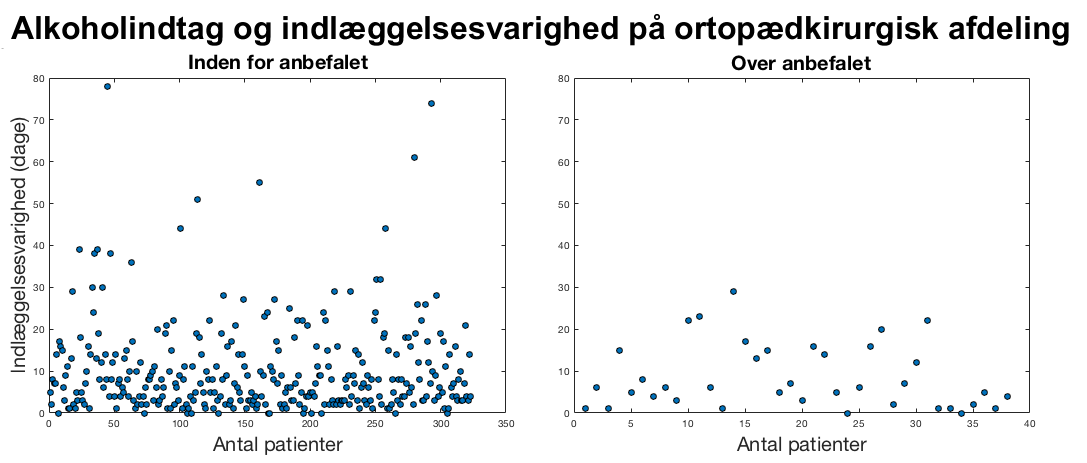
\includegraphics[scale=0.55]{figures/alkohologindlaeg}
	%\flushleft
	\caption{\textit{Alkohol og indlæggelsesvarigheden for patienter på ortopædkirurgisk afdeling. Alkohol er opdelt i inden for anbefalet og over anbefalet. Dette er over en periode på 3 måneder fra den 1. august til den 31. oktober år 2014. }}
	\label{alkohologindlaeggelse}
\end{figure}


\noindent
Det ses af \figref{alkohologindlaeggelse}, at størstedelen af patienter på ortopædkirurgisk afdeling befinder sig inden for anbefalingen af alkoholindtag. Den gennemsnitlige indlæggelsestid for patienter der holder sig inden for det anbefalede er 10 dage, mens den for patienter der drikker over anbefalet er indlagt 8,4 dage. Det tyder derfor på, at patienter der drikker inden for anbefalet er indlagt i længere tid. 

Det tyder på, at livsstilsfaktorer som komorbiditeter har betydning for indlæggelsesvarigheden. Patienter med komorbiditeter f.eks. dårligt blodomløb og diabetes kræver ofte særlig behandling. Diabetes har blandt andet betydning ift. sårheling \ref{interview}. Af figur \figref{diabetesogindlaeggelse} fremgår diabetes og indlæggelsesvarigheden. 

\begin{figure}[H]
	%\flushleft 
	\centering
	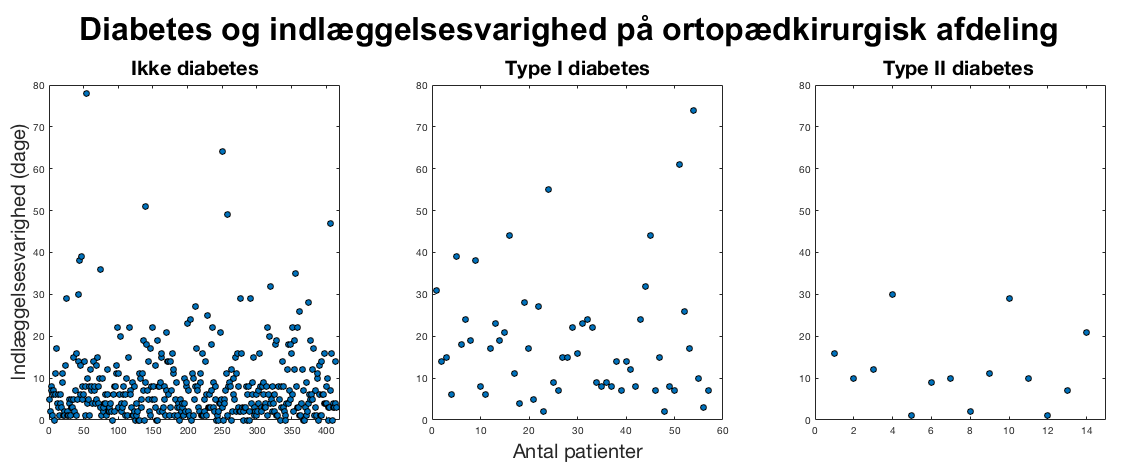
\includegraphics[scale=0.35]{figures/diabetesogindlaeg}
	%\flushleft
	\caption{\textit{Diabetes og indlæggelsesvarigheden for patienter på ortopædkirurgisk afdeling. Diabetes er opdelt i ikke diabetes, type 1 og type 2. Dette er over en periode på 3 måneder fra den 1. august til den 31. oktober år 2014. }}
	\label{diabetesogindlaeggelse}
\end{figure}

\noindent
På \figref{diabetesogindlaeggelse} fremgår det, at type 1 diabetikere har en længere indlæggelsesvarighed end type 2 diabetikere. Den gennemsnitlige indlæggelsesvarighed for ikke diabetikere er 7,8 dage, mens den gennemsnitlige indlæggelsesvarighed for type 1 og type 2 diabetikere er henholdsvis 18,8 og 12,1 dage. Det tyder derfor på, at der er en sammenhæng mellem diabetes og indlæggelsesvarigheden. 


\subsubsection{Indgreb}
Som beskrevet i \ref{kap_OA} udføres flere operationstyper med forskellig varighed på ortopædkirurgisk afdeling, hvorfor det forventes at indlæggelsesvarigheden ligeledes er varierende. 


\begin{figure}[H]
	%\flushleft 
	\centering
	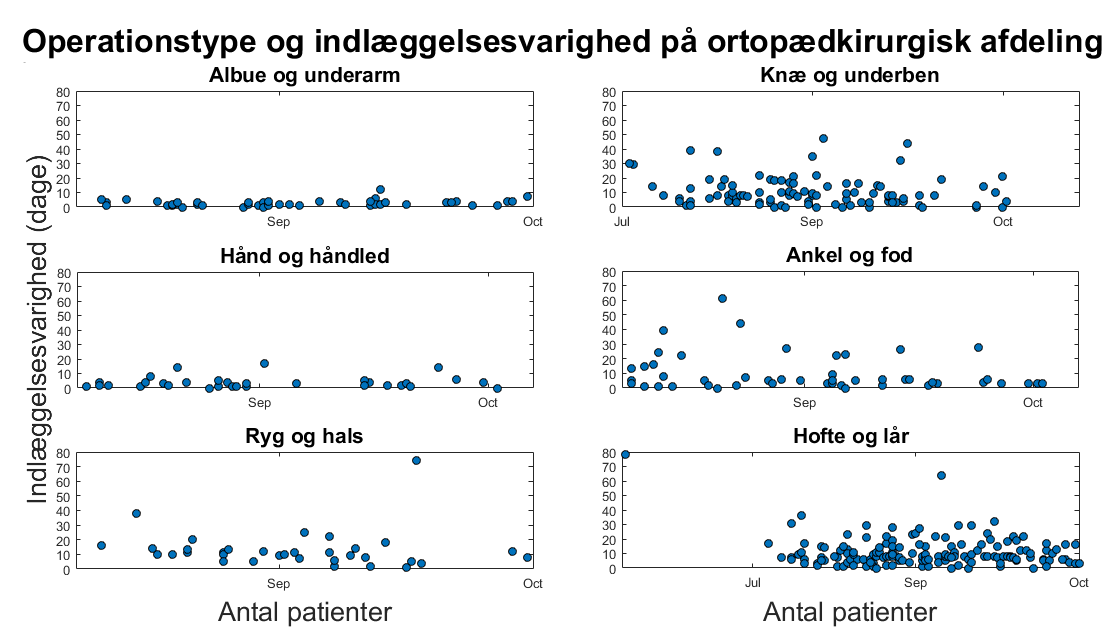
\includegraphics[scale=0.5]{figures/operaogindlaeg}
	%\flushleft
	\caption{\textit{Operationstyper og indlæggelsesvarigheden for patienter på ortopædkirurgisk afdeling. Operationstyper er opdelt efter albue og underarm, hånd og håndled, ryg og hals, knæ og underben, ankel og fod samt hofte og lår. Dette er over en periode på 3 måneder fra den 1. august til den 31. oktober år 2014.}}
	\label{opvsindlaegtid}
\end{figure}


\noindent
På \figref{opvsindlaegtid} fremgår det, at indlæggelsesvarigheden er varierende for typen af operation, hvoraf den gemmesnitlige indlæggesesvarighed er fra 2,7 dage op til 12,5 dage.  Den gennemsnitlige  indlæggelsesvarighed er for ryg og hals, hofte og lår, knæ og underben samt ankel og fod, henholdsvis 12,5, 10,8, 10,2 og 10,1 dage. Modsat er den gennemsnitlige indlæggelsesvarighed for hånd og håndled samt albue og underarm 3,8 og 2,7 dage. Hertil tyder det på, at indlæggelsesvarigheden er længere for operationer foretaget på underekstremiteter sammenlignet med overekstremiteter. Derudover ses det, at de fleste operationer der foretages på ortopædkirurgisk afdeling er en hofte og lår eller knæ og underben operation. 


\subsubsection{Tilgængelige kirurger}
Det kan i nogle tilfælde være nødvendigt at udsætte elektive patienters operationer, hvis et akut tilfælde opstår, hvorved kirurgen skal være til stede. Derved kan patienter indlæggelsesvarighed forlænges. Ved udsættelse af elektive patienter vil denne ofte få en ny tid hurtigst muligt. Den nye tid vil typisk være først på dagen, således risikoen for endnu en udsættelse mindskes.
\subsection{Postoperativt} \label{postop}
Udover præoperative faktorer kan der ligeledes opstå postoperative komplikationer, hvilket kan have indflydelse på en længere indlæggelsesvarighed for patienten. Postoperativt estimeres indlæggelsesvarigheden ligeledes ikke på nuværende tidspunkt, hvorfor der er taget udgangspunkt i informationspjecer fra ortopædkirurgisk afdeling på Aalborg Universitetshospital samt studier, der påviser komplikationer under og efter operaion.

\subsubsection{Komplikation under operation}
Det fremgår af afsnit \ref{praeop} at demografiske-, livsstils- og kliniske faktorer kan have indflydelse på komplikationer under operationer. Dette kan bl.a. være blødning og selve operationstypen. De statistiske tests påviste at alder, rygning, diabetes og operationstype har en statistisk sammenhæng med indlæggelsesvarighed. Da flere af disse faktorer kan medføre komplikationer under operationen og længere operationsvarighed, forventes det at det i nogle tilfælde kan være mere omfattende operationer, der kræver en længere operationsvarighed. Sammenhængen mellem operationsvarighed og indlæggelsesvarighed ses af \figref{opindlaeg}.


\begin{figure}[H]
	%\flushleft 
	\centering
	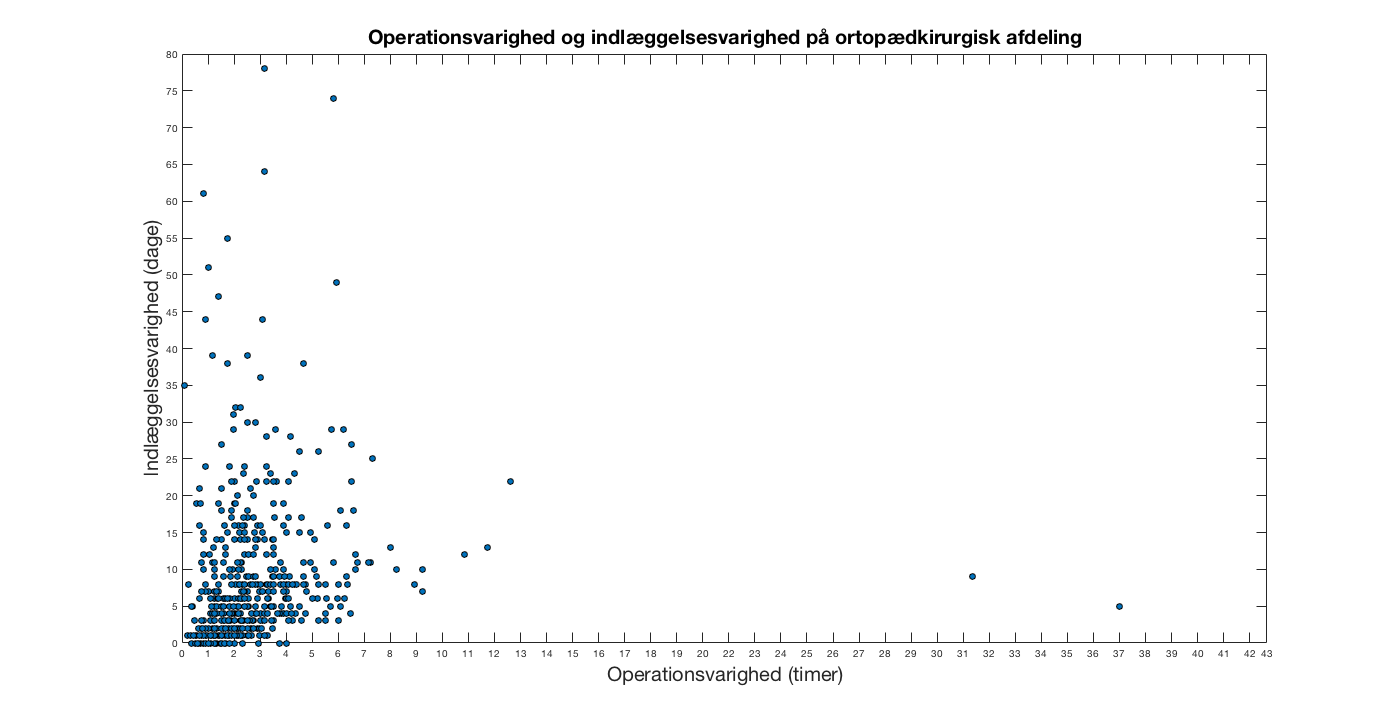
\includegraphics[scale=0.35]{figures/opindlaeg.png}
	%\flushleft
	\caption{\textit{Sammenhæng mellem operationsvarighed og indlæggelsesvarighed for patienter på ortopædkirurgisk afdeling. Dette er over en periode på 3 måneder fra den 1. august til den 31. oktober år 2014.}}
	\label{opindlaeg}
	\end{figure}

\noindent
På \figref{opindlaeg} fremgår det, at operationerne på ortopædkirurgisk afdeling tager op til 37 timer, hvoraf de fleste operationer varer 0 til 7 timer. Derudover ses det, at to operationer ved hhv. 31,5 time og 37 timer afviger fra de resterende operationsvarigheder. Den gennemsnitlige indlæggelsesvarighed er for patienter er 9,25 dage, mens den gennemsnitlige operationstid er på 3 timer. 

For at undersøge om der er en statistisk sammenhæng mellem indlæggelsesvarigheden og operationsvarighed udføres en korrelationstest. Resultatet af denne test kan fremgår af \tabref{opogindlaegtab}.

\begin{table}[H]
\centering
\begin{tabular}{|c|c|c|}
\hline
\textbf{}  & \textbf{Sub-sample} & \textbf{P-værdi} \\ \hline
\textbf{Indlæggelsesvarighed ift. operationsvarighed} & 486                 & 0,016*           \\ \hline
\end{tabular}
\caption{\textit{Korrelationstest for sammenhæng mellem indlæggelsesvarigheden og operationsvarighed. P-værdier under et signifikantsniveau på 5\% er angivet med *.}}
\label{opogindlaegtab}
\end{table}

\noindent
På \tabref{opogindlaegtab} ses p-værdien for sammenhængen mellem indlæggelsesvarigheden og operationsvarigheden, hvorved der fremgår en statistisk sammenhæng mellem indlæggelse- og operationsvarigheden. 

\subsubsection{Komplikationer efter operationen}
Efter en operation er det vigitgt at patienterne bevæger leddet hurtigst muligt, da dette er med til at mindske risikoen for komplikationer og smerter efterfølgende \ref{bilagA}\cite{Nordjylland2014}. Sammenhængen mellem træning og indlæggelsesvarigheden er illustreret på \figref{traeningindlaeg}.

\begin{figure}[H]
	%\flushleft 
	\centering
	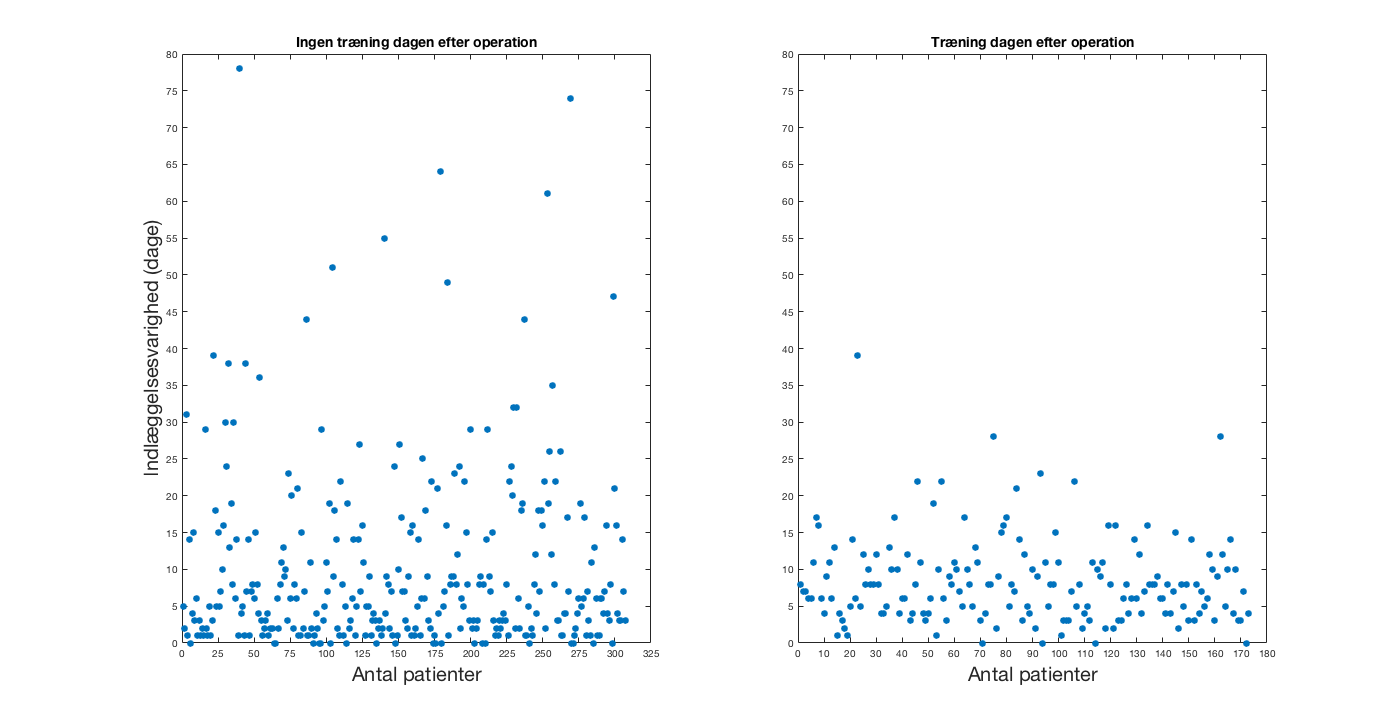
\includegraphics[scale=0.35]{figures/traeningindlaeg.png}
	%\flushleft
	\caption{\textit{Sammenhæng mellem træning og indlæggelsesvarighed for patienter på ortopædkirurgisk afdeling. Træning er opdelt i ingen træning dagen efter operation og træning dagen efter operation. Dette er over en periode på 3 måneder fra den 1. august til den 31. oktober år 2014.}}
	\label{traeningindlaeg}
	\end{figure}

\noindent
På \figref{traeningindlaeg} fremgår det, at der er flere patienter, som ikke træner dagen efter operationen. Ligeledes er variationen i indlæggelsesvarighed større for patienter, som ikke træner dagen efter end patienter der gør. Den gennemsnitlige indlæggelsesvarighed for patienter, der ikke træner dagen efter operation er 10 dage. Modsat er patienter, der træner dagen efter operationen 8,2 dage. Det tyder derfor på, at træning dagen efter operationen har en betydning for indlæggelsesvarigheden. 

For at teste om der signifikant sammenhæng mellem indlæggelsesvarighed og træning efter operationen udføres two sample t-test. Resultaterne heraf fremgår af \tabref{traeningindlaegtab}. 

\begin{table}[H]
\centering
\begin{tabular}{|c|c|c|c|}
\hline
\textbf{Træning efter operation}    & \textbf{Sub-sample} & \textbf{Indlæggelsesgennemsnit} & \textbf{P-værdi} \\ \hline
Ingen træning dagen efter       & 307                 & 9,95                            & 0,2248           \\ \hline
Træning dagen efter & 173                 & 8,24                            & 0,0950          \\ \hline
\end{tabular}
\caption{\textit{Statistik over sammenhæng mellem indlæggelsesvarigheden og træning dagen efter operation.}}
\label{traeningindlaegtab}
\end{table}

\noindent 
På \tabref{traeningindlaegtab} fremgår p-værdier for sammenhængen mellem indlæggelsesvarigheden og træning dagen efter operationen. Det ses ingen statistisk sammenhæng mellem indlæggelsesvarigheden og træning dagen efter operation.


\subsubsection{Udskrivelse af patienter}
Foruden komplikationer opstået hhv. under og efter operationen, kan afhentning af patienter ligeledes medføre en forlænget indlæggelsesvarighed. I nogle tilfælde kan patienter, der er klar til at blive udskrevet, være nødsaget til at ligge en dag ekstra på afdelingen, da de har brug for pleje i hjemmet efter operationen. Er hjemmepleje nødvendig, kræver det, at afdelingen kontakter kommunen før kl. 12 samme dag, hvis person, hvis personalet ikke når dette skal patienten være indlagt på afdelingen endnu et døgn. Derudover kan nogle patienter, der skal have efterbehandling eller genoptræning være nødsaget til at blive på afdelingen. Dette kan ligeledes gælde patienter, som i forvejen har komorbiditeter, hvor forandringer grundet operationen og indlæggelsen forværrer deres tilstand. Dette kan eksempelvis være demens, hvor patienten mister evnen til at varetage sit eget helbred. Disse patienter skal ofte vente på, at der er en aflastningsplads ledig før disse kan udskrives fra afdelingen. 



\chapter{Problemløsning}
På ortopædkirurgisk afdeling på Aalborg Universitetshospital ønskes der, på baggrund af afsnit \ref{kap}, en $100~\%$ kapacitetsudnyttelse med henblik på at udnytte de tilgængelige ressourcer optimalt. Kapacitetsudnyttelse er forholdet mellem aktivitet og kapacitet, hvoraf belægningsgraden er en betydende faktor ift. aktivitet. Det fremgår af afsnit \ref{omfang}, at belægningen på ortopædkirurgisk afdelingen er varierende, herunder opleves en ubalance i kapacitetsudnyttelse. Ved en belægning over $100~\%$ vil afdelingen opleve kapacitetsmangel, hvilket vil betyde at personalet skal yde mere end afdelingen har kapacitet til. Derimod vil afdelingen ved en belægning under $100~\%$ forårsage, at der ikke er fuld udnyttelse af personalets arbejdskraft. Da der ses ubalance i kapacitetsudnyttelsen og belægning kan dette tyde på, at der skal forekomme en effektivisering af planlægningen af patienter på ortopædkirurgisk afdeling. På baggrund af dette opstilles følgende hypotese:\\

\noindent
%\begin{itemize}
%\item 
Indlæggelsesvarigheden for patienter kan benyttes til at effektivisere kapacitetsudnyttelsen. 
%\end{itemize}

\subsection{Prædiktiv model}
For at forbedre kapacitetsudnyttelsen på ortopædkirurgisk afdelingen undersøges det, hvorvidt en prædiktiv model kan anvendes.
%Det fremgår af AFSNIT\fxnote{ref til afsnit}, at ortopædkirugisk afdeling på Aalborg Universitetshospital ikke fastholder en kapacitetsudnyttelse på $100$\%.\fxnote{snak sammen med Linette og Maria} 
Dette forventes muligt ved en forudsigelse af patienternes indlæggelsesvarighed. Aalborg Universitetshospital har i et tidligere projekt indsamlet data fra $1.000$ hospitalsindlæggelser fra ortopædkirurgisk afdeling. Disse data inkluderer bl.a. blodprøveanalyser og knoglescanninger (DXA), hvilket formodes at kunne anvendes til udvikling af en prædiktiv model. 

\noindent
Prædiktiv modellering definerer en proces, hvor en model udarbejdes med henblik på at forudsige hændelser. Denne model skal gøre det muligt at forstå og kvantificere nøjagtigheden af modellens forudsigelser ift. fremtidig data.\cite{Kuhn2013} 
Inden for sundhedssektoren er det muligt at prædiktere forskellige former for hændelser og forløb ved anvendelse af disse modeller. Dette kan eksempelvis være en forudsigelse om, hvorvidt en patient, indlagt med hjertestop, har risiko for endnu et hjertestop. Dette baseres på demografi, kost samt kliniske målinger. Et andet eksempel herpå kan være en estimering af glukosemængden i blodet hos en diabetiker, hvilket baseres på det infrarøde absorptionsspektrum af patientens blod.\cite{Hastie2008}

\noindent
Prædiktiv modellering kan opdeles i de to kategorier parametrisk og ikke-parametrisk. Forskellen på disse to kategorier ses overordnet ved om antallet af parametre kan varieres. I datasættet anvendt i projektet benyttes forskellige antal parametre for flere datapunkter og er derfor ikke-paramtetrisk.\cite{Sheskin2000}

\noindent
En prædiktiv model kan opbygges som en matematisk model eller en computerbaseret databehandlingsmodel (på engelsk: computational models). De matematiske modeller er mindre optimale at avende ved ikke-parametriske datasæt\fxnote{uddyb lidt måske}. Af denne årsag fokuserer projektet fremadrettet på computerbaseret databehandling, da denne egner sig bedst til det tilgængelige ikke-parametriske datasæt. \cite{Sheskin2000} 

\subsection{Indsamling af data}
Den prædiktiv model skal designes specifikt til ortopædkirurgisk afdeling på Aalborg Universitetshospital, da der er bestemte parametre som f.eks. operationer, procedurer, udstyr, personale og medicinering. For at sikre, at indsamling af data er tilstrækkelig og relevant skal der opstilles stramme retningslinjer for, hvordan disse indsamles og noteres. På baggrund af afgrænsningen til supervised learning i afsnit \ref{prae_model}, anses det nødvendigt, at hver indsamlede parameter kan have indflydelse for den enkelte patients indlæggelsesforløb. Disse overvejelser øger sandsynligheden for at opnå en brugbar prædiktiv model. 


%\subsection{Vurdering af parametre}
%Antallet af parametre vurderes grundlæggende ud fra parametrenes betydning for bestemmelse af indlæggelsesvarigheden. Flere parametre og mængden af data øger databehandlingstiden samtidig med, at modellen optager mere hukommelse i den anvendte computer.\cite{Kuhn2013}
%%Hvis computerkraft og budget ikke er den afgørende begrænsning i konstruktionen af en prædiktiv model, er det fordelagtigt at anvende så mange parametre som muligt for således at opnå en bedre estimering af indlæggelsesvarigheden.


%Da parametre kan angives som objektive og subjektive er det nødvendigt at finde en kvantificerbar skala til notering af parametrene. Objektive parametre som køn, alder og blodtryk angives med en direkte værdi. Subjektive parametre, som fysisk aktivitet og livsstil eksempelvis rygning, der oplyses af patienten. 
%


\subsubsection{Eksklusionskriterier for data} 
For at udarbejde en prædiktiv model opstilles kriterier ift. dataindsamling ud fra formålet med modellen. Da nogle modeller er sensitive for strømlinet data er det vigtigt at bestemme, hvorvidt der skal opstilles eksklusionskriterier til dataindsamlingen eller om en forudbestemt prædiktiv model skal anvendes.\cite{Kuhn2013}
For at systemet kan sammenholde parametre er det nødvendigt, at data er indskrevet efter faste retningslinjer. Hvis der ikke opstilles faste retningslinjer for indskrevet data, kan dette have indflydelse på estimeringen af indlæggelsesvarigheden.\cite{Kuhn2013} \\

\noindent
\textbf{Kategorisering af data} \\
\noindent
Ved at kategorisere data, anses det muligt at lave en prædiktiv model med en mindre mængde data. Denne model er dog ikke så specifik som en model uden kategoriseret data, da en mulig variation i parametrene kan reduceres.\cite{Rowan2007} 
Derfor bør det overvejes, hvor stor datamængden skal være for at konstruere modellens træningssæt. Ved ikke at kategorisere data, bliver modellen mere specifik ift. hver enkelt patient, men kræver dertil også en større database for at lave en funktionel model. Dette kan f.eks. inkludere meget specifikke kirurgiske indgreb eller sjældne komorbiditeter. 
Et eksempel på kategorisering af data kan være alder, hvor denne kan inddeles i aldersgrupper. En gruppe kan eksempelvis være 20-29 år hvilket kræver en mindre database, end aldersinddelingen 20-25 år, der udspænder et mindre interval.\cite{Rowan2007}  

\subsubsection{Opdatering af model}
En vigtig del af en prædiktiv model er, at denne kan tilpasse ændringer i parametres vægtning løbende ved ny data.\cite{Kuhn2013} Ved ændring i medicinering eller procedure af kirurgiske indgreb kan prædiktering af det gældende indgreb give misvisende estimateringer af indlæggelsesvarigheden. Derfor kan modellen ved transitioner mellem procedureændringer blive invalideret og dermed skal den prædiktive model have inkorporeret mere data før denne kan forudsige indlæggelsesvarigheden. 
Hvis et datapunkt ikke kan kategoriseres i systemet, kan det være nødsaget at ekskludere denne data fra indskrivelse i databasen.


\subsubsection{Præprocessering}
Hvis en datamængde allerede er tilgængelig, eksempelvis indsamlet til et andet formål, kan det være nødvendigt at anvende præprocessering på dataen. Dette gøres for at tilpasse den allerede indsamlede data til det nye formål.
Da flere parametre i datasættet fra ortopædkirurgisk afdeling på Aalborg Universitetshospital mangler, anses det nødvendigt at foretage præprocessering. Præprocessering foregår manuelt før en prædiktiv modellering kan foretages.
Der findes flere metoder, der kan anvendes for at kompensere for de manglende parametre. Kompenseringen kan forekomme ved kassering af værdier, tilegne manglende værdier, reducering af værdier og imputering. Imputering opdeles i tre underkategorier: Prædiktiv værdi imputation, Distribution-baserede imputation og Unik-værdi imputation. Prædiktiv værdi imputation erstatter den manglende værdi med estimerede værdier. Distribution-baserede imputation vægter værdien af manglende data mindre end det resterende, således disse får en mindre betydning under generering. Unik-værdi imputation erstatter den manglede værdi med en vilkårlig værdi fra samme parameter.\cite{Saar2007} 

Manglende data kan have flere årsager. Én årsag kan være manglende indsamlig af data grundet fejl. Manglende data kan også opstå som følge af andre faktorer. F.eks. kan udskrivelses tidspunkt være en manglende parameter hvis den pågældende person er død under indlæggelsen. Ligeledes kan manglende data være grundet censur, hvilket giver udtryk for en skjult ekstra parameter, eller som følge af en allerede kendt parameter.\cite{Kuhn2013} Dette fænomen er kendt som informative missingness. Da informative missingness betyder at manglende data er opstået som følge af en bestemt årsag, kan det være relevant ikke at imputere dataen, men derimod beholde den pågældende data. Derfor bør årsagen til hver manglende parameter overvejes, inden det besluttes hvorvidt der anvendes imputering, informative missingness eller en kombination af disse.
\section{Supervised machine learning}
Machine learning er en underkategori af kunstig intelligens og en metode, der kan anvendes til at genkende mønstre i data. Da machine learning anvendes på en computer, er det muligt at bearbejde datasæt af en størrelse, der er uhåndterbare for mennesker at behandle. Det bruges mange steder og har mange formål, som f.eks. søgemaskiner, forudsigelse af aktiekurser og ansigtsgenkendelse.\cite{DIKU2010}


Et computerprogram er essentielt et sæt regler, udarbejdet manuelt af en programmør. Dette regelsæt afgør hvordan programmet opfører sig. Et almindeligt program som dette kan ikke afvige fra sit regelsæt og er derfor begrænset til programmørens evner.
Supervised machine learning tager derimod udgangspunkt i input-output relationer, hvorved modellen uafhængigt er i stand til selv at danne et regelsæt. En illustration af dette fremgår af \figref{ml}.


\begin{figure}[H]
%	\flushleft
	\centering
	\includegraphics[scale=0.8]{figures/machinelearning.png}
%	\flushleft
	\caption{\textit{Machine learning danner et regelsæt ud fra input-output relationen.}\cite{DIKU2010}}
	\label{ml}
	\end{figure}


En udvidelse af databasen, hvoraf regelsættet dannes fra, kan modellen blive mere nøjagtig. Dette gøres i en logisk proces, kaldet induktiv inferens, hvilket er en metode, hvor computeren tilnærmer sandsynligheden for et givent output, ud fra en sammenligning med lignende eksempler. Der findes forskellige måder at gøre dette på, men fælles for alle undersøges det, hvorvidt den nye data ligner den eksisterende data.\cite{DIKU2010}


\subsection{Supervised machine learning til estimering af indlæggelsesvarighed}
Ubalancen i kapacitetsudnyttelsen på ortopædkirurgisk afdeling på Aalborg Universitetshospital ønskes afhjulpet. Indlæggelsesvarigheden afhænger af mange forskellige faktorer, hvorfor det er uoverskueligt for en koordinator at planlægge samtlige patienters indlæggelsesvarighed. På nuværende tidspunkt anvendes ingen redskaber til estimering af dette, hvilket resulterer i ubalance i forholdet mellem aktivitet og kapacitet, der udgør kapacitetsudnyttelsen på afdelingen. 


Det anses muligt at planlægge patienter efter deres indlæggelsesvarighed for således at opnå en balance i kapacitetsudnyttelsen. Da koordinatorer ikke kan overkomme alle parametre for patienter kan det være fordelagtigt at anvende en prædiktiv model som et redskab til at estimere indlæggelsesvarigheden. Ved at anvende supervised machine learning til denne model, kan skjulte sammenhænge mellem parametre samt en stor datamængde håndteres\cite{DIKU2010}.

\subsection{Konstruering af model}
Machine learnings modeller konstrueres som en algoritme på baggrund af indsamlet data.\cite{Kuhn2013}  Når en algoritme designes til machine learning gøres dette på baggrund af et træningssæt. \cite{DIKU2010} 


\subsubsection{Træningssæt}
Træningssættet tager udgangspunkt i en datamængde, der enten har kendte eller ukendte labels. Et træningssæt laves på baggrund af en del af den indsamlede data, hvor den resterende data testes på denne model. Et træningssæt basere på en forudbestemt machine learnings algoritme. Valget af algoritme belyses i afsnit \ref{algovalg}
Det er vigtigt at modellen ikke testes med samme data som anvendes til at opbygge træningssættet, da dette ville medføre at modellen kun er repræsentativ for den givne data.\cite{Kuhn2013} Ved supervised learning forsøges det at udarbejde en model, hvor data tilknyttes til labels og det bliver klassificeret. Det er vigtigt, at modellen afbildes så korrekt som muligt, for både træningssættet og de nye data. Et eksempel på udvælgelse af et træningssæts størrelse kunne være at udtage 200 datapunkter ud af 1000. Derefter konstrueres en algoritme på baggrund af træningssættet på 200 datapunkter, til at prædiktere en given parameter ud fra testsættet, hvilket er de resterende 800 datapunkter. Denne form for træningssæt opbygning er kendt som cross validation, og kan ses på figur \ref{fig:xval}\cite{Kuhn2013}.


\begin{figure}[H]
	%\flushleft 
	\centering
	\includegraphics[scale=.7]{figures/xval.png}
	%\flushleft
	\caption{\textit{Udvælgelse af datapunkter til træningssæt og testsæt.}\cite{Kuhn2013}}
	\label{fig:xval}
\end{figure}

\noindent
Ved at variere hvilken del af datapunkterne der anvendes til træningssættet er der mulighed for at opnå en lavere fejl i træningssættet, og dermed en højere præcision af prædikteringen.\cite{Kuhn2013} 


\subsubsection{Algoritme valg} \label{algovalg}
I sammenhæng med at cross validere træningssættet med den resterende data, testes forskellige machine learnings algoritmer for at opnå den ønskede grad prædikterings præcision.\cite{Kuhn2013} Valget af algoritme baseres på størrelsen af fejlen mellem træningssæt og testsæt, og vurderes på samme grundlag som træningssættet. Variationen af machine learnings modeller betyder at nogle modeller er mere idéelle til bestemte datasæt end andre. Eksempelvis kan C4.5 modellen håndtere manglende data, således at imputering kan undgås. Når en algoritme med den ønskede præcision mellem trænings- og testsæt er fundet påbegyndes det sidste trin i konstruktionen af den prædiktive model, at finde et passende antal parametre bygge konstruere modellen ud fra.\cite{DIKU2010}    

\subsubsection{Bestemmelse af parametre}
Når en prædiktiv machine learnings model konstrueres, er det essentielt at have det korrekte antal parametre fra træningssættet. For få parametre betyder at sandsynligheden for fejl ift. prædikteringen af den ønskede output parameter er høj.Ved for mange parametre sker en over-fitting, hvor modellen bliver så specifik for træningssættet, således at testsættet prædikteres upræcist.\cite{DIKU2010} Fejlraten i en prædiktiv model, generaliseringsfejlen, kan ses på figur \ref{fig:genfejl}.


\begin{figure}[H]
%	\flushleft 
	\centering
	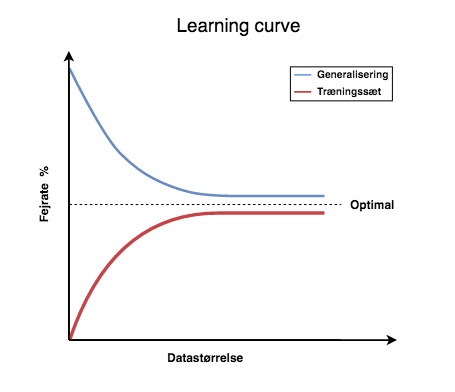
\includegraphics[scale=.8]{figures/genfejl.png}
	%\flushleft
	\caption{\textit{Learning curve der viser sammenhængen mellem datastørrelse og fejlrate.}\cite{Kuhn2013}}
	\label{fig:genfejl}
\end{figure}

\noindent
Generaliseringsfejlen bygges også på hvor stort trænings og testsættet er. Generaliseringsfejlen er dog eksponentielt faldende, og kan dermed ikke undgås helt, uafhængigt af træningsættets størrelse.\cite{DIKU2010}
Antallet af parametre, og hvilke der har størst indflydelse på outputtet testes ved at opbygge træningssæt med et begrænset antal parametre, og derefter prædiktere ud fra testsættet. Ved at anvende alle mulige kombinationer af parametre, kan der konstrueres en model. Denne model anvender de parametre der i sammenhæng har størst indflydelse på outputtet, med det lavest mulige antal parametre. Dermed kan machine learning anvendes til at vurdere hvilke parametre der har en statistisk sammenhæng, og bør inddrages i en model til eksempelvis prædiktering af indlæggelsesvarighed.\cite{Kuhn2013,DIKU2010} 

\urlstyle{same}

\printbibliography
\cleardoublepage

% BILAG
\begin{appendices}
\chapter{Bilag}

\section{Interview skabelon} \label{bilagA}
Dette bilag indeholder en skabelon for interview med sygeplejersker og en lægesekretær på ortopædkirurgisk afdeling på Aalborg Universitetshospital. Spørgsmål der ønskes svar på er angivet med fed skrift, mens formålet med spørgsmålet er angivet under. 

\subsection{Interviewet med sygeplejersker}
\textbf{Hvor mange arbejdstimer har du om ugen?} \\
\noindent
Der ønskes svar på: Gennemsnit, fordelingen af vagter uge for uge, længden af vagten, forskel på dag- og nattevagter, hvordan foregår vagtskifte. \\
\noindent
\textbf{Hvilke arbejdsopgaver har du på en normal vagt?} \\
\noindent
Der ønskes svar på: Hvor mange patienter sygeplejesker varetager. \\
\noindent
\textbf{Hvordan forløber dine pauser?} \\
\noindent
Der ønskes svar på: Sygeplejersker skal være til rådighed under pauser samt, hvorvidt denne er påtvungen. \\
\noindent
\textbf{Hvilke patienter modtager i på afdelingen?} \\
\noindent
Der ønskes svar på: Hvordan og hvorvidt patienterne skemalægges. Hvordan foregår indlæggelses og udskrivelse samt, hvorvidt der er nogle faste tidspunkter. Planlægges elektive patienter ud fra pladsen til akutte patienter.  \\
\noindent
\textbf{Hvor mange sengepladser har i til rådighed på afdelingen?}  \\
\noindent
Der ønskes svar på: Er der nogle sengepladser der er forbehold akutte patienter. \\
\noindent
\textbf{Hvad sker der, hvis i ikke har flere sengepladser til rådighed på afdelingen?} \\
\noindent
Der ønskes svar på: Hvor placeres patienterne, har afdelingen et samarbejde med andre afdelinger, er der prioritering mellem patienterne, fordeles patienterne mellem jer eller tilkaldes der ekstra personale, hvorfor opstår problemet og hvordan begrænser dette sygeplejerskerne, hvad gør de på afdelingen for at løse problemet udskydes elektive patienter. \\
\noindent
\textbf{Hvad sker der, hvis i har for mange sengepladser til rådighed?} \\
\noindent
\textbf{Er der en standardliste med checkpunkter af parametre som altid skal registreres for patienter?} \\
\noindent
Der ønskes svar på: Hvilke parametre sygeplejerskerne kigger på. \\
\noindent
\textbf{Er der noget du tænker, der er relevant at tilføje?} \\

\subsection{Interview med lægesekretær}
\textbf{Hvordan planlægges elektive patienter?} \\
\noindent
Der ønskes svar på: Planlægges patienter med kort eller lang varsel, estimeres der hvor længe patienten er indlagt med henblik på at planlægge elektive patienter forud, vurderes der specielle parametre i forhold til planlægningen. \\
\noindent
\textbf{Er der noget du tænker, der er relevant at tilføje?} \\





%\chapter{Bilag}

\section{Interviews med ortopædkirurgisk afdeling}
Dette bilag indeholder samtlige interviews foretaget på ortopædkirurgisk afdeling på Aalborg Universitetshospital. Interview med sygeplejersker fremgår af bilag \ref{bilag01} og bilag \ref{bilag02}, mens interviewet med lægesekretæren fremgår af bilag \ref{bilagsek}. Interviewer er angivet med fed skrift, mens informantens er angivet med kursiv skrift. 

\subsection{Sygeplejersker på sengeafsnit 01} \label{bilag01}
\textbf{Hvem er du?} \\
\noindent
\textit{Jeg hedder Mai Heilskov og jeg er sygeplejerske på O1, Aalborg sygehus syd. } \\
\noindent
\textbf{Og hvor længe har du været på afdelingen?}\\
\noindent
\textit{Snart 10 år} \\
\noindent
\textbf{Så vil vi høre om vi må citere dig for interviewet og optage?}\\
\noindent
\textit{ Ja, det må I gerne.}  \\
\noindent
\textbf{Her til at starte med så vil vi spørge om, hvor mange arbejdstimer har du om ugen?} \\
\noindent
\textit{34} \\
\noindent
\textbf{Så det er ikke fuldtids, men?} \\
\noindent
\textit{Ja, det svarer til at man har 3 dage fri på 8 uger eller sådan noget.} \\
\noindent
\textbf{Så du kører efter et 8 ugers vagtplan?} \\
\noindent
\textit{Al plan bliver kørt over de 8 uger, hvor det skal gå op i et antal timer.} \\
\noindent
\textbf{Okay, så det er 34 timers gennemsnit om ugen over 8 uger?} \\
\noindent
\textit{Ja.} \\
\noindent
\textbf{Så din vagtlængde det er 7,5 time? } \\
\noindent
\textit{8 eller 9 timers vagter.} \\
\noindent
\textbf{Okay, og det er dag og nat? Eller hvordan fungerer jeres skift?} \\
\noindent
\textit{Jeg kører dag-aften, men nogen kører dag-nat og nogle kører mere eller mindre primært nat eller aften.} \\
\noindent
\textbf{Så der er 3 vagtskift?} \\
\noindent
\textit{Der er 3 vagtskift.} \\
\noindent
\textbf{Okay, det passer med de 8 timer.} \\
\noindent
\textbf{Når du har her på en normal vagt, når du varetager patienter, hvor stor er en patient byrde? hvor mange patienter varetager du?} \\
\noindent
\textit{Hvor mange jeg har ansvaret for?} \\
\noindent
\textbf{Ja} \\
\noindent
\textit{Det er jo ikke primær pleje, så det er sådan lidt. Vi har tit gruppepleje, det betyder, at så er man jo 2 om et vis antal patienter. Men det varierer rigtig meget, hvor mange jeg har ansvaret for.} \\
\noindent
\textbf{Kan du sætte størrelse på, hvor mange I er sammen?} \\
\noindent
\textit{I dagvagt har vi måske typisk, er vi 2 om måske 6-8 patienter. sådan typisk alt efter om vi har overbelægning eller ej, men deromkring. I aftenvagten er vi jo 2 om 10-12 patienter.} \\
\noindent
\textbf{Nu siger du overbelæning, er det når i har?} \\
\noindent
\textit{Mere end de 20 patienter vi er normerede til.} \\
\noindent
\textbf{Okay, så det er når i har mere end de 20 normerede sengepladser. } \\
\noindent
\textbf{I forhold til dine pauser, hvordan forløber de? Kan I blive indkaldt i jeres pauser? eller har I påtvunget, at I skal holde pauser?} \\
\noindent
\textit{Pauserne, det er når det passer ind i forhold til arbejdsrytmen og nogen dage er der ikke pauser.} \\
\noindent
\textbf{Og man kan blive indkaldt fra sine pauser?} \\
\noindent
\textit{Ja, vi har jo telefon. Vi har sådan nogle dæktelefoner på os, så læger kan ringe til os og vi kan blive kaldt på med opkald fra gangen, fra patienter og sådan noget.}
\textbf{Så i er disponible?} \\
\noindent
\textit{Vi er disponible.} \\
\noindent
\textbf{Fra I møder til I går hjem?} \\
\noindent
\textit{Ja, det er vi.}  \\
\noindent
\textbf{Når I modtager patienter på afsnittet, de elektive patienter, skemalægges det ift. de indlægges på et bestemt tidspunkt eller?
Informant: De planlagte operationer?} \\
\noindent
\textit{Ja, de planlagte.} \\
\noindent
\textit{De kommer typisk om morgenen, fordi de planlagte operationer er jo i dagstid. så det kun, hvis det er den første på programmet, og de bor langvejsfra, så kan de komme dagen før nogen gange. så kommer de måske typisk kl 8 om aftenen.} \\
\noindent
\textbf{Så de bliver indskrevet måske et halvt døgn før indgrebet?} \\
\noindent
\textit{Ja.} \\
\noindent
\textit{Heroppe nogle gange og nogle gange på patienthotellet, det er sådan nyt, at der er nogen der går der ned. Og så kommer de så herop om morgenen, nogle gange kommer de her alligevel.} \\
\noindent
\textbf{Og de akutte patienter de indskrives døgnet rundt?} \\
\noindent
\textit{ Ja, det gør de.} \\
\noindent
\textbf{Er der et bestemt tidsrum I udskriver patienter på? Er der et tidspunkt på døgnet I ikke udskriver patienter på?} \\
\noindent
\textit{Langt de fleste udskrivelser foregår måske mellem 12 og 16, medmindre de er planlagt dagen før, så kan det være om formiddagen. Men det er jo typisk, fordi der først er stuegang kl 9, det er først der lægerne kommer, så 9, kvart over 9. Så før at man får kørt stuegang igennem og de praktiske ting er klar før personen kan komme hjem, så det typisk over middag før de kan. } \\
\noindent
\textbf{Hvor ofte vil du sige, at man vurderer patienternes tilstand, hvornår de kan sendes hjem?}  \\
\noindent
\textit{Altså det vurderer vi jo dagligt i forhold til, hvad vi tænker er realistisk i forhold til hvornår de skal hjem. og tager jo egentligt relativt hurtigt i forløbet af patienterne stilling til, hvad de tænker, og så sender vi jo, hvis de skal have hjælp, plejeforløbsplan afsted. sådan at de kan udskrives.} \\
\noindent
\textbf{Så det vurderes i starten, hvor lang tid kommer de til at ligge og så når det nærmer sig det tidsrum de skulle ligge, så vurderer man så igen?} \\
\noindent
\textit{Ja.} \\
\noindent
\textbf{Fint. Så er det om der er nogen tidspunkter I ikke indlægger patienter. Nu siger du, at akutte patienter kan komme døgnet rundt, men er der nogen tidspunkter I vagtskifter, at I venter?} \\
\noindent
\textit{Nej. De kommer, når det passer fra skadestuen af.} \\
\noindent
\textbf{De elektive patienter, der så er planlagte, hvordan foregår det, når der kommer en akut patient og tager vedkommendes sengeplads? Bliver de udsat?} \\
\noindent
\textit{Det er sjældent de er akut, fordi tit så er det forskellige stuer de bliver opereret på. og de planlagte elektive patienter kører jo på nogle andre stuer og kører rent dagtid. Så derfor så er det sjældent der er et overlap i forhold til de to. Det er mere nogen akutte patienter, der er derhjemme, der bliver kaldt ind til nogle operationer, hvor at der måske er noget der er endnu mere akut, der så kommer og tager deres plads.} \\
\noindent
\textbf{Okay.} \\
\noindent
\textit{Men elektive patienter de kører som regel på nogle andre stuer, så skal der være massiv overbelægning, så bliver de aflyst og så bliver de aflyst allerede måske hjemmefra.} \\
\noindent
\textbf{Så inden de ankommer, så får de en ny tid?} \\
\noindent
\textit{Ja.} \\
\noindent
\textbf{Det var også i forhold til jamen, hvor mange sengepladser har i forbeholdt til akutte i forhold til elektive, om der er en fast procentsats?} \\
\noindent
\textit{Ikke jeg er helt bekendt med i hvert fald.} \\
\noindent
\textbf{Okay. Hvad sker der så, hvis i ikke har flere sengepladser til rådighed? Du siger overbelægning, i ikke har plads til mere end 20 senge i har heroppe, hvad gør I så med patienterne, der kommer, de akutte?} \\
\noindent
\textit{Vi har jo lidt ekstra pladser. Vi er normeret til de 20 patienter, det er det vi har personale til, men vi har 22-24 antal fysiske pladser, hvor de kan være, så det fylder vi jo så op først. Men vi er jo to sengeafdelinger, så det hedder sig, at man fylder op til normeringen og det har vi antal pladser til og så kører den anden afdeling op til normeringen og de har plads til 25 ovre på den anden side af gangen på O2, så det er først når begge afsnit er fyldt helt op med normeret, så fylder vi jo ekstra og vi har begge steder et par ekstra fysiske pladser, hvor folk kan være. vi har bare ikke personale.} \\
\noindent
\textbf{Til at varetage?} \\
\noindent
\textit{Ja. Derefter så kommer de så på gangen, hvis det er, at vi ikke kan sørge for overflytning til andre steder på det tidspunkt.} \\
\noindent
\textbf{Så når du siger andre steder, så mener du?} \\
\noindent
\textit{Andre matrikler, altså vi har Farsø, og vi har Hjørring og vi har Frederikshavn.} \\
\noindent
\textbf{Okay, så i gør det ikke lokalt, i flytter dem ud på andre ortopædkirurgiske matrikler?} \\
\noindent
\textit{Okay, alt efter hvor specialet er og om der er plads de steder, men det jo primært mandag til fredag det er en mulighed. De fleste andre steder har ikke kirurgiske pladser så, hvis de akutte patienter, der kommer, hvor der er behov for operation. Det har de ikke i weekenden de andre steder, så er det jo her på Aalborg, men så forsøger vi så at flytte nogle af dem der måske er færdigbehandlet, der kan komme til videre genoptræning eller videre mobilisering til andre matrikler. } \\
\noindent
\textbf{Fint.} \\
\noindent
\textit{Så har vi også geriatriske pladser jo.} \\
\noindent
\textbf{En gang til?} \\
\noindent
\textit{Vi har sådan nogle geriatriske pladser, altså vi har jo 6 ortopædkirurgiske geriatriske pladser over på geriatriskafsnit, der har vi 6 pladser der, jeg kan ikke huske om det er 4 eller 6 pladser til ortopædkirurgiske patienter, så der har vi vores hoftepatienter der også kommer derover. Det aflaster jo så også os nogen gange.} \\
\noindent
\textbf{Det kan i også aflaste på.} \\
\noindent
\textit{Ja.} \\
\noindent
\textbf{Så i forhold til, nu siger du, at I får flere patienter end Ier normeret senge til. Og det i forhold til personalet som sagt?} \\
\noindent
\textit{Ja.} \\
\noindent
\textbf{Hvad gør i så? Nu har vi ud fra noget litteratur fundet ud af, at I tilkalder noget ekstra vagtpersonale fra vikarbureau eller hvordan foregår det? } \\
\noindent
\textit{Altså det er jo altid en vurderingssag, det jo ikke altid antallet af patienter, men også tyngden af de patienter der er fordi at, hvis det er overbelægning med 4 relativt ukomplicerede håndkirurgiske patienter, hvor de skal ind og have sat skinner i og så går de hjem og man forventer de går hjem samme dag, så er det ikke nødvendigvis man får en ekstra ind. Mens, hvis det nogen der er plejekrævende eller hvis det er rigtig mange håndpatienter også oveni sammen med de andre, så kommer der ekstra vikarer ind. }\\
\noindent
\textbf{Så det er i forhold til speciale eller hvor lang tid de skal?} \\
\noindent
\textit{ Hvad vi også forventer i forhold til, hvornår de skal hjem.} \\
\noindent
\textbf{Okay, så du vil sige generelt, hvis I har problemer på afdelingen når I har for mange patienter, så det personalemangel, der først begrænser jer før plads og udstyr eller?} \\
\noindent
\textit{De mangler jo altid udstyr, så der jo borde, hvis de er på gangen så har jo ingen borde og sådan nogle ting og de har jo ikke noget strøm og ingen skabe de kan låse ting indeni.} \\
\noindent
\textbf{ Nu snakker jeg også om i forhold til behandlingsudstyr eller genoptræningsudstyr.} \\
\noindent
\textit{Vi har det vi har, men mange de får jo hjælpemidler op i forhold til, hvis det er længere og det kommer nede fra hjælpemiddeldepotet og sådan nogle ting, så det er ikke nødvendigvis ikke, hvor mange patienter man har. } \\
\noindent
\textbf{Så nu kom du ind på tidligere, at I også får patienter fra det andet ortopædkirurgisk afsnit herinde, hvis i har en plads her og de mangler plads, men er der andet i gør, hvis i har sengepladser til rådighed? End at tage patienter fra den anden ortopædkirurgiske afdeling? } \\
\noindent
\textit{Vi skal nok få dem fyldt op. } \\
\noindent
\textbf{Okay, så i plejer at få dem fyldt op? } \\
\noindent
\textit{Ja, sådan relativt hurtigt i hvert fald, fordi så kommer de planlagte jo også. Altså jeg var her i går aftes og der var vi jo, vi er normerede til de 20, vi startede med at have 16 patienter eller 17, men da jeg gik hjem, havde vi fået patient nr. 20, så vi var op på det normerede faktisk til midnat, men jeg vidste der kom 3 patienter ind til morgen plus 2 der skulle ringes ind, så vi vidste jo, at vi ville jo komme op over det normerede.} \\
\noindent
\textbf{Så i vidste allerede, at I skulle begynde at aflaste på den anden afdeling og få udskrevet patienter?} \\
\noindent
\textit{Ja} \\
\noindent
\textbf{Okay. Nu er det i forhold til noget med, når I går ind og vurderer, hvor lang tid skal man lægge her om der noget bestemt I går ind og vurderer det ud fra, indlæggelsesvarigheden af patienterne?} \\
\noindent
\textit{ Ja det gør vi jo, men det er alt efter hvad speciale, hvad de fejler, hvad de har fået lavet.}  \\
\noindent
\textbf{Så det er ud fra diagnose og operation?} \\
\noindent
\textit{Ja og grundsygdom, altså grund diagnoser. Man kan jo godt ved nogen sige, at de er meget komplicerede. Man ved det kommer til at tage et længere indlæggelsesforløb.
Interviewer: Men der er ikke noget systematisk tjekliste i skal igennem eller er det bare vurderingssag?} \\
\noindent
\textit{Vi ved, at ca et normalt hoftepatient, der får et brud og der falder, det tager typisk omkring de 5 dage, så vi melder dem hjem til efter de 5 dage efter en operation og så kan man jo justere det bagefter jo.} \\
\noindent
\textbf{Så det er baseret på erfaring?} \\
\noindent
\textit{Ja.} \\
\noindent
\textbf{Er der nogle parametre, der vægter mere end andre? } \\
\noindent
\textit{I forhold til?} \\
\noindent
\textbf{I forhold til indlæggelsesvarigheden?} \\
\noindent
\textit{Mobiliseringsgraden inden er ret væsentligt. Hvad vi forventer af dem fordi, hvis det er en plejehjælpsbruger, der næsten ingen gangfunktion har inden, har vi ikke en forventning om at vi kan gøre det bedre. Så hvis de har været vant til at bruge lift nærmest inden,  så er det også den forventning vi har. Hvis de bor på plejehjem, kommer de også typisk hjem tidligere fordi der er fysioterapeuter koblet på plejehjemmene, så der får de den mobilisering og genoptræning på plejehjem i stedet for. } \\
\noindent
\textbf{Nu siger du det her med at komme hjem. Oplever I, når I skal sende patienter hjem, at der nogle gange opstår prop i forhold til, at patienterne skal udskrives og ældre patienter skal til plejehjem eller hvordan foregår det? } \\
\noindent
\textit{Der er sjældent, når de skal tilbage til plejehjemmet, hvis de bor på plejehjem. Problemet er tit, hvis de bor i et hjem, der simpelthen ikke er egnet til måske de hjælpemidler de skal bruge eller et hjem, der ikke kan rumme de nødvendige forandringer der er nu eller at nogen der har egentlig taget været lidt demente og de har egentlig taget kunnet klare sig, men så sker der forandringer, når de bliver indlagte og de bliver meget konfuse og meget demente. Det eskalerer nærmest deres sygdom, så de kan ikke komme hjem til sig selv. Der oplever vi tit en flaskehals fordi at så skal vi vente på en aflastningsplads til dem. Det kan godt være lidt svært at få til mange af dem.} \\
\noindent
\textbf{Så det er generelt ældre, der er problemet med at få hjem?} \\
\noindent
\textit{Ja, eller det er mere problemet, hvis de skal have en aflastningsplads. Det er tit der, der sker en flaskehals.}  \\
\noindent
\textbf{Så er der lige her til slut, er der andet du tænker, der er et problem på afdelingen i forhold til, at I måske står og mangler personale eller noget der forsinker jer i jeres arbejdsdage?} \\
\noindent
\textit{Jamen, selvfølgelig er der altid problemer nogle gange, når vi er for lidt personale, hvis der er sygdom eller noget andet, der gør at vi er for få hænder til at udføre arbejdet. Men det er nogengange den indstilling man har til det. Jeg tror, at jeg er meget positivt indstillet sådan generelt, så det er jo en udfordring, men ikke en begrænsning for at jeg kan komme igennem dagen og det stresser mig ikke nødvendigt, men det kan det jo godt gøre ved mange, hvis man konstant ligger med overbelægningsprocent, der er forhøjet. Vi ser jo også perioder, hvor der er flere der går hjem med stress pga. det. } \\ \noindent
\textbf{Så stress er en faktor på afdelingen? det er noget der påvirker jer?} \\
\noindent
\textit{ Ja.} \\
\noindent
\textbf{Nu hvor du på forhånd siger, at du vidste der ville være for mange patienter her i dag til morgen, vælger i så at tilkalde folk, altså ekstra personale på forhånd eller løber I bare hurtigere? } \\
\noindent
\textit{Vi er inde og vurdere. Vi er inde og kigge på, hvor mange er vi sat på til vagten i dag og der var egentlig taget sådan rimeligt antal personale sat på til at være i dag.
Hvis det havde været en dag, hvor der var for få personale sat på, så havde vi måske forsøgt at kalde på en. Men de havde også kaldt på en her, vi har en ekstra personale i dag.} \\
\noindent
\textbf{Okay, men er det lokalt fra afdelingen eller et vikarbureau? } \\
\noindent
\textit{ Det endte så med at være en over fra O2, fordi de så ikke havde så mange patienter, så der har vi lånt en herover. } \\
\noindent
\textbf{Så I har den der synergi, at i arbejder sammen med hinanden?} \\
\noindent
\textit{Vi forsøger.} \\
\noindent
\textbf{Ja, I forsøger.} \\
\noindent
\textit{Men altså, hvis de har rigtig mange patienter, så er vi også nogen gange ovre og hjælpe dem i både dagvagt og aftenvagter også for at forsøge at hjælpe hinanden i hvert fald.} \\
\noindent
\textbf{Det er i orden. Tak for interviewet.} \\


\subsection{Sygeplejerske på sengeafsnit 02} \label{bilagO2}
\textbf{Til at starte med vil vi så spørge, hvem er du?}\\
\noindent
\textit{Jeg hedder Lars og er almindelig sygeplejerske på gulvet.}\\
\noindent
\textbf{Hvor længe har du arbejdet på denne her afdeling?} \\
\noindent
\textit{$28$ år.}\\
\noindent
\textbf{Må vi citere dig for det her interview?}\\
\noindent
\textit{Ja det må I godt.}\\
\noindent
\textbf{Til at starte med at høre, hvor mange arbejdstimer har du gennemsnitligt om ugen?}\\
\noindent
\textit{Almindelig fuldtidsstilling, $37$ timer.}\\
\noindent
\textbf{Hvor lang tid er det fordelt over ift. om det er gennemsnitligt for en måned eller om det er gennemsnit hver uge?}\\
\noindent
\textit{Vi har en arbejdsplan, der hedder otte uger i alt, hvor jeg så veksler mellem dagvagter og aftenvagter.}\\
\noindent
\textbf{Har i så vagtskifte, når du siger dag og nat. Er der nogle bestemte tidspunkter de her vagtskifte finder sted?}\\
\noindent
\textit{Ja, på alle mine hverdage, dagvagter, arbejder jeg fra $7$ til $15$:$45$, og så møder jeg aftenvagten ind lidt tidligere. De møder ind $15$:$30$, så de har et kvarter til at sætte sig ind i de patienter de skal, og imens de gør det, skal jeg passe klokker.}\\
\noindent
\textbf{Så I får ligesom aflastet og sagt, at det er de her patienter I skal varetage og får fordelt viden.}\\
\noindent
\textit{Ja, men det er meningen, at de skal sætte sig og læse. Og jeg skal kun sige noget, hvis der er noget jeg lige skal af med, ellers skal de læse sig til det. Plus jeg skal tage klokkerne ude på gangen.}\\
\noindent
\textbf{Hvor mange patienter varetager du på en normal vagt? Har I et bestemt antal patienter, der er tildelt?}\\
\noindent
\textit{Nej, det er forskelligt, fordi de veksler meget i sværhedsgraden eller hvordan vi passer dem og selvfølgelig, hvad de fejler - to til fire til seks patienter.}\\
\textbf{Så det er to til seks på området.}\\
\noindent
\textit{Ja.}\\
\noindent
\textbf{Så kommer der noget ift. pauser. Nu har vi læst, at I har nogle pauser, hvis I har de her arbdejdsdage, om de er betalte pause, altså om I kan blive indkaldt I jeres pauser? eller hvordan det foregår?}\\
\noindent
\textit{Det ved jeg faktisk ikke, altså jeg bliver altid indkaldt, nu går vi med de her telefoner.  Så hvis lægen vil have fat i mig, så ringer han, fordi vi har skrevet os på tavler dernede med, at jeg har de patienter. Så har jeg mit navn og denne her telefon, så kan de ringe efter mig, hvis det er, eller fysioterapeuten, eller min kollega, hvis der er nogen. Så der er ikke sådan faste pauser. Man kan altid finde en. I hvert fald ikke mere, det kan godt være, at det har været sådan. Jeg tror også godt man må sige, man går til pause, men kutymen er, at man rejser sig, hvis der er brug for det. Plus det er også vores kloksystem, og det vil sige, jeg kan se, hvis jeg sidder ude og får kaffe, så ringer telefonen eller også, hvis jeg ikke har min telefon, så kan jeg se på en display, om det er min patient, der ringer både på stuen, men også ude på toilettet. Kutymen er, at hvis vi er et par stykker om de samme patienter. Èn af os tager klokken. Det er ikke meningen, at de andre skal tage den.}\\
\noindent
\textbf{Så patienterne er fordelt og tildelt mellem jer?}
\noindent
\textit{Ja.}
\noindent
\textbf{Så er det lidt ift., når I modtager de her patienter. Nu har vi snakket lidt med sekretariatet ift., hvordan I modatager de her patienter. Er det et bestemt tidsrum, du ser, at I modtager de her patienter? Nu snakker vi ift. de elektive patienter dem, der er planlagt om der er et bestemt tidsrum?}\\
\noindent
\textit{Det er der sådan set ikke helt, fordi vi får også afhængig af, hvad dage det er, patienter om eftermiddagen, der skal gøres klar til næste dag. Men altså indkaldte patienter møder om morgenen typisk kl $7$. Det er der også en sat af til at tage imod, så de bliver taget fra ude foran ved sekretæren, også kommer de ind på deres plads og så stiller man de spørgsmål, der er relevante og så sørger man for, at de er klædt om og parat til operationen, hvis de skal ned allerede ved 8-tiden eller lidt senere.}\\
\noindent
\textbf{Så i modtager dem om morgen og gør dem klar til i løbet af dagen?}\\
\noindent
\textit{Ja, det gør vi ved de fleste patienter.}\\
\noindent
\textbf{Så er det ift. de akutte patienter, det er døgnet rundt I modtager dem?}\\
\noindent
\textit{Ja, her på afdelingen.}\\
\noindent
\textbf{Ift. udskrivelse af patienter, foregår det et bestemt tidsrum på dagen, hvor man siger vi udskriver patienter fra kl. $10$ til kl. $14$, ellers udskriver vi ikke eller hvordan foregår det?}\\
\noindent
\textit{Det er også meget forskelligt, fordi dels, så kommer de fra kæmpe optagområder og nogen kommer endnu længere væk fra, så tit er det transporten, der nogengange bestemmer, hvornår vedkommende bliver hentet og alt afhængig af, hvem der henter dem. Hvis det er Falck og de skal hjem eller hvis de skal til et andet sygehus, så har de et tidsrum på to timer eller fire timer. Hvis du bestiller en taxa, så kan du næsten få et klokketidspunkt indenfor fem minutter. Og det synes jeg faktisk, at de er gode til at overholde.}\\ 
\noindent
\textbf{Så I udskriver løbende som der er behov for det?}\\
\noindent
\textit{Ja.}\\
\noindent
\textbf{Så ift., når I vurderer om patienter kan udskrives, hvor ofte gøres det? Er det ift., når der er stuegang eller er det flere gange i løbet af dagen eller hvordan vurderes det?}\\
\noindent
\textit{Nej, altså vi har jo et. Det er jo meget forskelligt for vores patienter, fordi vi har små børn og vi har unge mennesker og ældre mennesker og så har vi de rigtig gamle. De unge mennesker eller børn kan godt have en operation, hvor man skal have fat i hjemmesygeplejersken til at source dem, og det skal være planlagt i god tid. Også de andre, der aftaler man typisk over computeren om, hvordan man udskriver dem, og hvordan man sender dem hjem.}\\
\noindent
\textbf{Hvor ofte vurderer man så, hvornår de skal hjem og hvornår de er klar. Er det en dialog med patienten eller?}\\
\noindent
\textit{Ja, men typisk skal hjemmeplejeren også være blandet ind i det, og de skal komme til dem, så vil de helst have de ikke kommer for sent, fordi der er jo også forskel på deres dagvagt, hvor de er flest på arbejde. Og så kommer man over i en aftenvagt, hvor de ikke er ret mange på arbejde. Så det gælder om at få dem hjem i dagstiden. Det er meget vigtigt.}\\
\noindent
\textbf{Okay. Så ift. om der er nogle tidspunkter, hvor I ikke længere udskriver patienter og indlægger patienter f.eks. om natten?}\\
\noindent
\textit{Ikke indlægger, fordi vi er en akut afdeling. Der tager vi alt, hvad der kommer. Og udskriver, vi kan godt have en trafikulykke, hvor vi tror, at der er en hel masse, men hvor det hele bliver afviklet eller det hele bliver godkendt, at patienten ikke fejler noget. Og det kan typisk være en knallertulykke eller en bilulykke, hvor man kommer ind og kommer til observation. Det kan være om eftermiddagen eller det kan også være først på aftenen, hvor lægen kommer op og vurderer patienten og siger du fejler ikke noget og du må have lov til at komme hjem, men det er deres afgørelse.}\\
\noindent
\textbf{Nu siger du lægen? Er det læger, der vurderer patienterne, der kommer ind akut eller er det en kirurg?}\\
\noindent
\textit{Altså jeg har kun kirurger på min afdeling, og jeg må ikke som sygeplejerske sende nogen hjem på eget initiativ.}\\
\noindent
\textbf{Så de skal have været forbi?}\\
\noindent
\textit{En læge skal have godkendt og jeg skal i kontakt med en læge på en eller anden måde for at spørge om vedkommende må komme hjem, og det kan også være et barn med en brækket arm, der er opereret i løbet af formiddagen eller eftermiddagen, som hvis de ellers har det godt med smerter og ingen kvalme, så må man gerne have lov til at sende dem hjem om aftenen, hvis lægen siger god for det og det kan godt være pr. telefonen.}\\
\noindent
\textbf{Nu kommer vi ind på noget ift. sengepladser. Har I nogle sengepladser som I altid forbeholder til akutte patienter ift., når I fordeler sengene?}\\
\noindent
\textit{ Nej, det kan vi ikke mere, fordi vi har rimelig mange patienter til daglig, og vi er faktisk også begyndt og lade være med tænke på, at der ligger to eller tre mænd på en stue eller kvinder. Nu bruger vi simpelthen bare de pladser vi har, så vi ikke skal flytte rundt. En kvinde kan godt overnatte sammen med to mænd fordi vi har forhæng for.}\\
\noindent
\textbf{Så der er noget diskretion?}\\
\noindent
\textit{Ja. Og så er der nogle, der bliver flyttet om næste dag.}\\
\noindent
\textbf{Nu kommer vi nemlig ind på det her med, hvis der ikke er sengepladser nok på de her værelser, og du siger, at I godt kan finde på at placere dem bare inde på stuerne. Er I nødt til at have patienter liggende på gangen nogen gange? Nu det ikke natten over, nu det bare i løbet af dagen?}\\
\noindent
\textit{Ja, det har vi gjort tidligere, men brandvæsnet er efter os. Vi må ikke. For nogle år tilbage der var vi fuldstændig fyldt op. Også alle vores patienter har jo på en eller anden måde næsten brug for et hjælpemiddel af en slags. Det kan være krykker, de fylder ingenting, men gangstativ, kørestole, bækkenstole, hvad ved jeg. Alt fylder og det hele det kom herop til os, så det står heroppe til den enkelte patient med navn på. Det stod engang ude på gangen, det må det ikke for brandtilsynet. Så kom vi det ind på stuerne, så kom vi de ekstra patienter, du snakker om, de akutte, de blev stående ude på gangen. De må det ikke. Så kørte vi dem ind, så siger brandtilsynet, det er patienternes sikkerhed, så der skal vi køre patienterne ind på stuerne, hvis der er brand f.eks. og hjælpemidlerne må vi simpelthen bare placere i et andet rum. Det er ligegyldigt hvad, der må ikke være noget på gangene. Og det gjorde så, at vi fra, for et par år siden, hvor vi normalt har fire sengestue, sagde så vil vi kun have tre sengestuer for at have tre patienter på stuen, men så have et hjørne til alle hjælpemidlerne. Det kan vi sådan nogenlunde holde.}\\
\noindent
\textbf{Så I har valgt at sige nu tager vi det her udstyr og flytter det ind på stuen?}\\
\noindent
\textit{Ja, og hvis nummer fire patienter kommer, så får vedkommende pladsen og så skal vi finde et andet sted til udstyret.}\\
\noindent
\textbf{Jamen så er det lidt ift., hvis I så får for mange patienter, altså akutte patienter, og I ikke kan placere dem på de her stuer, da de er fyldt op. Hvad gør I så? Nu har vi læst, at der er trådt nogle regler i kraft med, at de bliver flyttet ned til andre stuer og andre afdelinger og om du kan bekræfte det?}\\
\noindent
\textit{Ja, det bliver så bare styret et andet sted fra. Det bliver styret fra AMA, Akut medicinsk modtagerafsnit. Der sidder nogle koordinatorer, som skal sørge for, at deres patienter der ovre fra eller fra modtagelsen, det medicinske regi, at der er plads til dem dvs., hvis de medicinske afsnit ikke har pladser nok, så kan vi risikere, at skal have en medicinsk patient eller to og det sørger den koordinator for.} \\
\noindent
\textbf{Så det er ikke jer, der styrer de patienter, og hvordan de flyttes?}\\
\noindent
\textit{Nej, vi skal melde tilbage. Jeg ved ikke om vi skal i dagligdagen, men i weekenderne, der skal vi melde tilbage. Jeg tror det er inden kl. 11 ellers så er det omkring kl. $9$ til koordinatoren og sige, at vi har to ledige pladser ellers forventer vi to ledige pladser lidt senere over middagen eller sådan noget, også har de råderum over dem i princippet.}\\
\noindent
\textbf{Ja, indtil I får en akut patient, der overtager.}\\
\noindent
\textit{Ja, så finder vi så ud af, hvad vi skal gøre. Det er lige trådt i kraft.}\\
\noindent
\textbf{Okay. Så, hvis I har nogle af de her ekstra patienter ift. hverdage, så bliver I sat på arbejde til at udfylde stuen eller udfylde afdelingen ift., hvor meget personale, der møder op eller hvordan fungerer det?}\\
\noindent
\textit{Nej, altså der jo planlagt, hvem der møder ind på den der otte ugers plan, så de skal bare møde ind, og så skal vi fordele patienterne, når vi kommer om morgenen. Og det har vi så gjort ved, at vi har typisk fire fem specialer, og de specialer har vi valgt os ind på af egen interesse, så jeg har, i en lang periode, så skal jeg passe rygpatienter primært. Men det kan godt være, at jeg skal passe børn, og det kan også være jeg skal passe noget andet eller noget tredje eller medicinske patienter. Det er forskelligt fra dag til dag. Men vi prøver at koncentrere os om dem vi har valgt os ind på.}\\
\noindent
\textbf{Ja, fordi det lidt ift., hvis der kommer for mange patienter og I ikke kan varetage dem, så har vi læst, at I har et vikarbureau I kontakter og får noget ekstra personale ind, og det kan du bekræfte, at det er sådan det fungerer?} \\
\noindent
\textit{Ja sådan set, hvis vi er i nød, så må vi ringe.}\\
\noindent
\textbf{Ja også ift. overarbejde om det er noget I bliver meget påvirket af altså, at I bliver nødt til at blive ekstra, når I for eksempel har de her vagtskifte, at I bliver nødt til at blive ekstra for at hjælpe det nu kommende vagthold?}\\
\noindent
\textit{Nej, det synes jeg ikke er noget problem. Det er meget sjældent.}\\
\noindent
\textbf{Okay, så det er sjældent det sker.}\\
\noindent
\textit{Ja, fordi så er det mig det hænger på eller de to andre, fordi vi er der jo til at lappe over. De resten er jo taget hjem, så der er kun tre at trække på, hvis der er nogle som ikke møder op eller vi har overset noget, eller der er et eller andet akut.}\\
\noindent
\textbf{Nu har vi har arbejdet med det her med, at I nogle gange har for mange patienter eller for lidt personale på arbejdet. Hvad er det, der først begrænser jer, er det, at I mangler plads på afdelingen eller er det, at I ikke har nok personale eller hvornår er det de her stress situationer opstår?}\\
\noindent
\textit{Altså det er sjældent vi har for mange patienter. Vi kan godt have mange patienter, men det behøver altså ikke være for mange, men det er nærmere, at vi ikke er nok personale til dem vi har af patienter, fordi mange af vores patienter kræver meget. Altså og kræver meget der mener jeg, at det tager lang tid at gøre ting færdige.}\\ 
\noindent
\textbf{Ja, altså passe og plejer?}\\
\noindent
\textit{Ja, passe og pleje og sørge for at tingene er i orden som det nu skal være, hvis det er helt rigtigt.}\\
\noindent
\textbf{Så det er ikke det fysiske, at det er pladsen heroppe, der mangler og at det er udstyret, men det er mere personalemangel nogen gange ift. opgavebyrden?}\\
\noindent
\textit{Ja, til opgavebyrden. Det er nok det rigtige ord. Det er fordi der mange, lige på min afdeling, at vi har nogle, hvor ting vitterligt tager lang tid og det bliver værre og værre, og der kommer flere og flere af den slags patienter ind fordi folk bliver ældre.}\\
\noindent
\textbf{Og det du siger er rygafdeling eller rygpatienter.}\\
\noindent
\textit{Ja, men vi har også mange med sår. Også har de ældre mennesker kommer typisk med andre skavanker, hvor det også tit er det vi skal tage os af, fordi det kan være sukkersyge eller dårlig blodomløb, hvor de kommer ind med et lille sår på en tå som vi skal tage os af.}\\
\noindent
\textbf{Så, når I har nogle elektive patienter og nogle akutte patienter, og når de her akutte patienter kommer og jeres arbejdsbyrde bliver større, løber I så bare hurtigere og gøre jeres arbejde hurtigere?}\\
\noindent
\textit{Ja.}\\
\noindent
\textbf{Udskyder I så de her elektive patienter og siger, at vi kan først operere jer i morgen eller hvordan fungerer det?}\\
\noindent
\textit{Ja, det kan sagtens tænkes. Men det er ikke os som sygeplejerske eller social og sundhedsassistent, der bestemmer det. Det er rent lægeligt administrativt.}\\
\noindent
\textbf{Okay, det er administrativt?}\\
\noindent
\textit{Ja. Man kan godt sige, at vi er spændt for, sådan rent teknisk eller administrativt, så kører det op på et lidt andet plan.}\\
\noindent
\textbf{Så er det ift., når I får de her patienter ind, vurderer I, hvor lang tid skal de ligge?}\\
\noindent
\textit{Nej, lad os sige kun rygpatienterne. Der vil jeg sige der har vi, hvis det er planlagt, så har vi, at det tager en uge f.eks., men nogle gange der går lidt længere tid, fordi der er ting der ikke lige går efter kalenderen, men ellers passer det nogenlunde. Men vi har mange sårpatienter, hvor det går langt over tiden fordi vi efterhånden er så specialiserede lægeligt og fordi vores afdeling er en sårafdeling så får vi alt, altså så får vi alle de patienter, der fejler noget med deres sår i en eller anden forbindelse.}\\
\noindent
\textbf{I forbindelse med vores projekt, går vi ind og kigger på om der er nogle parametre I går ind og vurderer. Nu siger du, vi har, hvis der er noget med ryggen, så ved I, at det tager en uge. Men er der noget andet f.eks. et skema I skal gå efter, hvor der er nogen ting I skal krydse af altså, hvor gammel er patienten er eller?}\\
\noindent
\textit{Nej, lige specielt rygsektoren har jo gjort sig god ved, at det er så systematiseret, at det er de samme kategorier end en skæv ryg på en ung pige. Der kommer næsten en hver $14$. dag, og de bliver jo opereret på samme måde og bliver passet på samme måde af fysioterapeuterne som kommer med det samme, så vi er hele tiden i gang med dem, så det forløb er planlagt til en uge.}\\
\noindent
\textbf{Okay, så det er vurdering ud fra erfaring simpelthen?}\\
\noindent
\textit{Ja, og ligesådan, vi har mange cancerpatienter, der kommer, hvor de pludseligt ikke kan mærke deres ben,  tværsnitssyndrom hedder det. De bliver også opereret sådan og sådan. Forløbet er sådan og sådan. De  skal op, de skal i gang og de skal holdes vedlige. Vi skal ikke presse dem, men vi skal sørge for, at de holder sig i gang.}\\
\noindent
\textbf{De skal være aktiverede?}\\
\noinden
\textit{Ja, hvorimod folk, der bliver amputeret, det er en anden kategori patienter, fordi de har tit dårligt blodomløb, sukkersyge, dårligt syn. Altså de er ikke så nemme at køre på den måde. Der skrider det hele.}\\
\noindent
\textbf{Så der er forskellige parametre indenfor hver kategori?}\\
\noindent
\textit{Ja meget.}\\
\noindent
\textbf{Og det er baseret på erfaring og ikke noget dokumenteret system?}\\
\noindent
\textit{Nej, det har jeg i hvert fald ikke styr på. Men rygsektoren det kører på de firkantede kasser og det kører bare.}\\
\noindent
\textbf{Så er det kun her til sidst om der er noget du har lyst til at tilføje eller noget du har lyst til at fortælle ift. jeres arbejde heroppe?}\\
\noindent
\textit{Nej, men det nye er, at man skriver til kommunen med udskrivelser og det gør man i så god tid som muligt, også kan man hele tiden rette på computeren, hvad man har skrevet eller hvad ens kollega har skrevet, så de hele tiden er opdateret.}\\
\noindent
\textbf{Så det er lidt det der nogengange begrænser jer heroppe, at det er svært at komme af med patienten bagefter eller?}\\
\noindent
\textit{Nej, hvis man er ude i god tid og får det skrevet ordentligt, og det ikke fordi, at man skal skrive så meget fordi det også blevet sådan et kasse system. Man skal bare huske det. Der er nogle gange vi glemmer det.}\\
\noindent
\textbf{Også, når der kommer akutte patienter?}\\
\noindent
\textit{Ja, men det er alligevel, at man skal skrive til kommunen, at man gør det og så nogle gange, hvis vi har lidt travlt, og man skal skrive det dagen før inden kl. $12$, tror jeg. Og hvis jeg først skal ind nu og skrive det nu, altså nu er kl. $13$. Se så skal jeg beholde patienten en dag mere.}\\
\noindent
\textbf{Så det er på den måde det foregår?}\\
\noindent
\textit{Ja, men der er så noget jeg ikke har helt styr på endnu, men der er noget, som hedder udskrivningsenheden. Jeg ved ikke om de sidder og kigger på, hvad jeg har skrevet, men når jeg så melder dem til i morgen eller i overmorgen, så ved jeg ikke om de sidder og kontrollerer og ringer til kommunen. Det har jeg ikke styr på.}\\
\noindent
\textbf{Når I flytter patienterne rundt, nu siger du, hvis I har en akut patient, så får de lov til at ligge på gangene først eller ryger de ind på stuen?}\\
\noindent
\textit{De ryger ind på stuen.}\\
\noindent
\textbf{Så prioriterer man så at få flyttet nogle af dem, der senere i deres helingsforløb eller elektive patienter ud eller?}\\
\noindent
\textit{Aldrig ude på gangen.}\\
\noindent
\textbf{Okay, det er ned på andre stuer eller?}\\
\noindent
\textit{Ja, så kan vi finde på det.}\\
\noindent
\textbf{Okay, så det er de elektive patienter og dem der er mindst kritiske akutte som I flytter ned på andre afdelinger?} \\
\noindent
\textit{Nej, ikke andre afdelinger. Det gør vi ikke så meget af, men vi kan godt finde på at flytte en patient fra vores afdeling over på vores naboafdeling, som også er en ortopædkirurgisk afdeling. I dagligdagen er vi delt op i to forskellige ting. Det hedder stadigvæk det samme og det er det samme. Der veksler vi hele tiden mellem patienterne, når det er de akutte, fordi om aftenen så kan de godt have travlt, hvor vi så tager deres patienter og næste dag, så er der faldet lidt ro over det, så hører de til derovre og så flytter vi dem derover. Men vi flytter dem ikke på en mave afdeling eller en medicinsk afdeling. Det er ikke det der foregår, men det vi snakkede om lige før med AMA, der har rådighed over hele sygehuset.}\\
\noindent
\textbf{Er der forskel på, hvordan man prioriterer de her patienter? Og hvem man flytter eller er det forskelligt?}\\
\noindent
\textit{Ja, der er det blevet sådan, at vi passer på børnene og vi passer på rygpatienter og vi passer på traumepatienter. Hvis der kommer nogle med hoftebrud, det er sådan blevet en folkesygdom. De hører til ovre på den anden afdeling, men dem passer vi også, hvis de ikke kan eller har tid til det, og har plads til dem. Men vi sender helst ikke børn over og vi må ikke sende rygpatienter over. Førhen hed det også knogle konstruktion, som også er meget specielt på vores afdeling. Dem vil vi heller ikke have andre steder, fordi det er sådan noget, hvor vi forlænger benene med noget apparatur og der er kun nogle få læger, som er her og de vil ikke have dem andre steder hen, fordi så skrider det hele og så går der noget galt med deres udstyr og varetagning. Det er ligesådan med rygpatienter. De vil altså helst have, at de er her, for de har oplevet, det er også det med erfaring. De har sendt folk ud af huset, hvor det andet sygehus ikke har varetaget det som de skulle eller har kørt deres eget system, så ødelægger det noget for patienten, også kan de måske starte forfra og det vil de ikke have mere.}\\ 
\noindent
\textbf{Så vil vi sige tak for interviewet.}\\
\noindent
\textit{Velbekomme.}\\



\section{Lægesekretær} \label{bilagsek}
\textbf{Vi kunne godt tænke os at høre om, hvem er du?}\\
\noindent
\textit{Jeg hedder Janni Ulstrup og jeg er lægesekretær her i ortopædkirurgisk afdeling i idrætsklinikken.} \\
\noindent
\textbf{Og hvor længe har du arbejdet her?} \\
\noindent
\textit{Det har jeg i fire år.} \\
\noindent
\textbf{Fire år?} \\
\noindent
\textit{Ja. Og så har jeg været i ortopædkirurgien, 7 år tidligere i min tid som lægesekretær.} \\
\noindent
\textbf{Og må vi citere dig for interviewet?}\\
\noindent
\textit{Ja.} \\
\noindent
\textbf{Jamen nu vil jeg spørge, hvordan planlægger I de her elektive patienter?}\\
\noindent
\textit{Vi har faste pladser. Vi har ikke så mange elektive under indlæggelse, men vi har rigtig mange elektive i dagkirurgi. I dagkirurgi har vi rigtig mange tider og  holder altid nogle enkelte ledige til, hvis der dukker noget akut op under indlæggelse. Det er kun de patienter, der er absolut nødvendigt skal opereres under indlæggelse, der kommer derind og det er ikke altid vi faktisk udnytter alle vores tider. I denne her uge har vi for eksempel ikke brugt vores pladser som vi så har været heldige med fordi der har været mange akutte patienter, så de har haft meget overbelægning eller mange patienter deroppe, så det har faktisk været heldigt i denne her uge. Men dem planlægger vi sådan, at vi som regel altid har plads til lidt ekstra. Vi booker ikke stramt op, kun i absolut nødstilfælde og det er, hvis der kommer en ekstra en på som man er nødt til at skal have plads til.}
\textbf{Er der en procentsats eller en del af sengene, der er afsat til akutte patienter?}\\
\noindent
\textit{Nej det tror jeg ikke. Ikke mig bekendt. Altså vi må operere om tirsdagen for vores vedkommende og der må vi sætte en til to patienter på afhængigt af, hvor stort et indgreb det er. Det er af hensyn til operationsgangen og deres kapacitet der. Det er egentligt ikke af hensyn til sengeafdelingen. Det er en del af vores elektiv. Det ved de, at der kan komme to, hvis det er to små operationer. Men en del af de patienter vi sender op på sengeafdelingen, selvom de er nødt til at skulle opereres under indlæggelse, så er det måske noget i forhold til anæstesi sikkerhed og opvågning. Mange af de patienter kan måske godt allerede gå hjem senere på dagen. Det er ikke nødvendigvis ensbetydende med, at de skal ligge deroppe i flere dage. Men der er også dem, der så kommer der op fordi de netop skal ligge der i nogle dage, fordi de skal træne efter operationen. Der er ikke som er 100 procent fastlagt.} 
\textbf{Når I indkalder de her elektive patienter, bliver det så gjort med kort eller lang varsel? Hvordan foregår det?}\\
\noindent
\textit{Jamen, hvis der sidder en patient henne i ambulatoriet i dag, der skal opereres under indlæggelse, så vil patienten få en tid med hjem i dag. Og hvis det ikke er noget, der haster og hvis det ikke er noget akut, så finder vi første ledige tid under de omstændigheder der nu er. Skal det være en bestemt læge, er det patienten, der siger jeg vil gerne vente til efter 15. December eller under de forhold, der nu er der. Er det sådan at patienten siger første ledige tid, jamen så vil de simpelthen få første ledige tid og det kan godt være i næste uge. Det kan også være om 14 dage, tre uger.}
\textbf{Hvis så man er nødt til at rykke den elektive patient under akutte patienter, hvordan gør man så?}\\
\noindent
\textit{Det er igen et spørgsmål om for vores område fordi vi ikke er så stramt booket op under indlæggelse. Så har vi plads til, at vi kan putte dem på måske en uge, måske 14 dage senere. Altså vi får dem på forholdsvis hurtigt og vi skal nok sørge for, at de får en tid. Vi kan også løbe ind i perioder, hvor vi har mange, der skal ligge under indlæggelse. Og så kan vi selvfølgelig godt løbe ind i kniberi med, hvad gør vi så her. Og så er det egentligt vores specialeansvarlige overlæge, der træder ind og siger, jamen så gør vi sådan her. Så er det ham, der ligesom træffer beslutningen om, hvordan håndterer vi det.} 
\textbf{Når I indkalder de her patienter, planlægger de elektive patienter, planlægger I så også efter for eksempel operationstype, hvor lang tid skal de ligge der?}\\
\noindent
\textit{Nej.} \\
\noindent
\textbf{Er der noget du føler er relevant lige at tilføje.} \\
\noindent
\textit{Nej, ikke andet end det her er jo kun for sengeafdelingen. Vores O6 kører jo ligesom et forløb for sig selv. Det er ambulant kirurgi. Det kører ligesom sit liv for sig selv, men der har vi også altid buffer, hvis der er nogen, der bliver aflyst. Vi prøver på at have en regel om, at den første tid bliver som regel ikke booket. Det er den vi holder tilbage, fordi det sjældent, at det er den første patient man aflyser, hvis man aflyser, så opererer man som regel de patienter, der er mødt ind i dagkirurgi. Så vælger man at aflyse dem der endnu ikke er mødt. Dem der først kommer senere på dagen. Så på den måde, hvis der er nogen, der bliver aflyst i dag og de så får en tid på mandag fra morgenstunden af, jamen så møder de ind, så bliver de opereret, så man undgår, at de bliver aflyst mere end én gang. Men hvis vi sætter dem på senere på dagen, så kan vi risikere, at de rent faktisk bliver aflyst en gang mere, hvis det skulle være. 7-9-13 og bank under bordet, det sker heldigvis ikke ret tit, men det kan jo ske på grund af sygdom.} \\
\noindent
\textbf{Bare lige om jeg har forstået det korrekt, så snakker du noget om, at I ud fra, når I planlægger, så planlægger I om, altså ud fra om kirurgen også, om den er tilstede den dag det skal være, så det gør I ud fra erfaring og operationstype.}\\
\noindent
\textit{Det er ud fra, det er lægen selv, der har skrevet på. Lægen udfylder en operations tilmelding nu når de skriver patienter op til operation og derpå skriver han skal jeg selv operere denne her patient eller kan det være en anden der gør det. Patienten får også selv lov at vælge og sige jamen ønsker du, at det skal være den læge. Hvis ikke han har skrevet noget på, så får patienten selv lov at vælge. Jamen jeg vil gerne have, at det var den eller nej, jeg vil bare gerne have så hurtig en tid jeg kan få.} \\
\noindent
\textbf{Okay, så det er de overvejelser I gør, når det er?}\\
\noindent
\textit{Ja, det er ligesom vores sygeplejersker, der sidder og har papirene og siger jamen vi skal have en tid, der passer ind med det her, men patienten vil bare gerne ind så hurtigt som muligt. Det kan også godt nogen gange være, at lægen skriver han gerne selv vil gøre det, men hvis der går et stykke tid og patienter siger jeg vil bare gerne have det overstået, så kan man måske godt sige okay, fint nok. Det er ikke noget, der er noget specielt kompliceret i, så det vil en anden også godt kunne gøre, det her.}


\end{appendices}
\end{document}
